\documentclass[twoside]{book}

% Packages required by doxygen
\usepackage{calc}
\usepackage{doxygen}
\usepackage{graphicx}
\usepackage[utf8]{inputenc}
\usepackage{makeidx}
\usepackage{multicol}
\usepackage{multirow}
\usepackage{fixltx2e}
\PassOptionsToPackage{warn}{textcomp}
\usepackage{textcomp}
\usepackage[nointegrals]{wasysym}
\usepackage[table]{xcolor}

% Font selection
\usepackage[T1]{fontenc}
\usepackage{mathptmx}
\usepackage[scaled=.90]{helvet}
\usepackage{courier}
\usepackage{amssymb}
\usepackage{sectsty}
\renewcommand{\familydefault}{\sfdefault}
\allsectionsfont{%
  \fontseries{bc}\selectfont%
  \color{darkgray}%
}
\renewcommand{\DoxyLabelFont}{%
  \fontseries{bc}\selectfont%
  \color{darkgray}%
}
\newcommand{\+}{\discretionary{\mbox{\scriptsize$\hookleftarrow$}}{}{}}

% Page & text layout
\usepackage{geometry}
\geometry{%
  a4paper,%
  top=2.5cm,%
  bottom=2.5cm,%
  left=2.5cm,%
  right=2.5cm%
}
\tolerance=750
\hfuzz=15pt
\hbadness=750
\setlength{\emergencystretch}{15pt}
\setlength{\parindent}{0cm}
\setlength{\parskip}{0.2cm}
\makeatletter
\renewcommand{\paragraph}{%
  \@startsection{paragraph}{4}{0ex}{-1.0ex}{1.0ex}{%
    \normalfont\normalsize\bfseries\SS@parafont%
  }%
}
\renewcommand{\subparagraph}{%
  \@startsection{subparagraph}{5}{0ex}{-1.0ex}{1.0ex}{%
    \normalfont\normalsize\bfseries\SS@subparafont%
  }%
}
\makeatother

% Headers & footers
\usepackage{fancyhdr}
\pagestyle{fancyplain}
\fancyhead[LE]{\fancyplain{}{\bfseries\thepage}}
\fancyhead[CE]{\fancyplain{}{}}
\fancyhead[RE]{\fancyplain{}{\bfseries\leftmark}}
\fancyhead[LO]{\fancyplain{}{\bfseries\rightmark}}
\fancyhead[CO]{\fancyplain{}{}}
\fancyhead[RO]{\fancyplain{}{\bfseries\thepage}}
\fancyfoot[LE]{\fancyplain{}{}}
\fancyfoot[CE]{\fancyplain{}{}}
\fancyfoot[RE]{\fancyplain{}{\bfseries\scriptsize Generated on Sun Jul 27 2014 19\+:45\+:39 for Occluded Library by Doxygen }}
\fancyfoot[LO]{\fancyplain{}{\bfseries\scriptsize Generated on Sun Jul 27 2014 19\+:45\+:39 for Occluded Library by Doxygen }}
\fancyfoot[CO]{\fancyplain{}{}}
\fancyfoot[RO]{\fancyplain{}{}}
\renewcommand{\footrulewidth}{0.4pt}
\renewcommand{\chaptermark}[1]{%
  \markboth{#1}{}%
}
\renewcommand{\sectionmark}[1]{%
  \markright{\thesection\ #1}%
}

% Indices & bibliography
\usepackage{natbib}
\usepackage[titles]{tocloft}
\setcounter{tocdepth}{3}
\setcounter{secnumdepth}{5}
\makeindex

% Hyperlinks (required, but should be loaded last)
\usepackage{ifpdf}
\ifpdf
  \usepackage[pdftex,pagebackref=true]{hyperref}
\else
  \usepackage[ps2pdf,pagebackref=true]{hyperref}
\fi
\hypersetup{%
  colorlinks=true,%
  linkcolor=blue,%
  citecolor=blue,%
  unicode%
}

% Custom commands
\newcommand{\clearemptydoublepage}{%
  \newpage{\pagestyle{empty}\cleardoublepage}%
}


%===== C O N T E N T S =====

\begin{document}

% Titlepage & ToC
\hypersetup{pageanchor=false,
             bookmarks=true,
             bookmarksnumbered=true,
             pdfencoding=unicode
            }
\pagenumbering{roman}
\begin{titlepage}
\vspace*{7cm}
\begin{center}%
{\Large Occluded Library \\[1ex]\large 0.\+1 }\\
\vspace*{1cm}
{\large Generated by Doxygen 1.8.7}\\
\vspace*{0.5cm}
{\small Sun Jul 27 2014 19:45:39}\\
\end{center}
\end{titlepage}
\clearemptydoublepage
\tableofcontents
\clearemptydoublepage
\pagenumbering{arabic}
\hypersetup{pageanchor=true}

%--- Begin generated contents ---
\chapter{Hierarchical Index}
\section{Class Hierarchy}
This inheritance list is sorted roughly, but not completely, alphabetically\+:\begin{DoxyCompactList}
\item \contentsline{section}{occluded\+:\+:buffers\+:\+:attributes\+:\+:attribute}{\pageref{classoccluded_1_1buffers_1_1attributes_1_1attribute}}{}
\item \contentsline{section}{occluded\+:\+:buffers\+:\+:attribute\+\_\+buffer}{\pageref{classoccluded_1_1buffers_1_1attribute__buffer}}{}
\begin{DoxyCompactList}
\item \contentsline{section}{occluded\+:\+:buffers\+:\+:interleaved\+\_\+attr\+\_\+buffer}{\pageref{classoccluded_1_1buffers_1_1interleaved__attr__buffer}}{}
\item \contentsline{section}{occluded\+:\+:buffers\+:\+:segregated\+\_\+attr\+\_\+buffer}{\pageref{classoccluded_1_1buffers_1_1segregated__attr__buffer}}{}
\end{DoxyCompactList}
\item \contentsline{section}{occluded\+:\+:buffers\+:\+:attribute\+\_\+buffer\+\_\+factory}{\pageref{classoccluded_1_1buffers_1_1attribute__buffer__factory}}{}
\item \contentsline{section}{occluded\+:\+:buffers\+:\+:attributes\+:\+:attribute\+\_\+map}{\pageref{classoccluded_1_1buffers_1_1attributes_1_1attribute__map}}{}
\item \contentsline{section}{occluded\+:\+:scene\+:\+:objects\+:\+:camera}{\pageref{classoccluded_1_1scene_1_1objects_1_1camera}}{}
\begin{DoxyCompactList}
\item \contentsline{section}{occluded\+:\+:opengl\+:\+:retained\+:\+:scene\+:\+:objects\+:\+:gl\+\_\+retained\+\_\+camera}{\pageref{classoccluded_1_1opengl_1_1retained_1_1scene_1_1objects_1_1gl__retained__camera}}{}
\begin{DoxyCompactList}
\item \contentsline{section}{occluded\+:\+:opengl\+:\+:retained\+:\+:scene\+:\+:objects\+:\+:gl\+\_\+retained\+\_\+fixed\+\_\+camera}{\pageref{classoccluded_1_1opengl_1_1retained_1_1scene_1_1objects_1_1gl__retained__fixed__camera}}{}
\end{DoxyCompactList}
\end{DoxyCompactList}
\item \contentsline{section}{occluded\+:\+:utilities\+:\+:files\+:\+:file\+\_\+reader}{\pageref{classoccluded_1_1utilities_1_1files_1_1file__reader}}{}
\item \contentsline{section}{occluded\+:\+:opengl\+:\+:retained\+:\+:gl\+\_\+attribute\+\_\+buffer}{\pageref{classoccluded_1_1opengl_1_1retained_1_1gl__attribute__buffer}}{}
\item \contentsline{section}{gl\+\_\+retain}{\pageref{classgl__retain}}{}
\item \contentsline{section}{occluded\+:\+:opengl\+:\+:retained\+:\+:gl\+\_\+retained\+\_\+object\+\_\+manager}{\pageref{classoccluded_1_1opengl_1_1retained_1_1gl__retained__object__manager}}{}
\item \contentsline{section}{occluded\+:\+:meshes\+:\+:mesh}{\pageref{classoccluded_1_1meshes_1_1mesh}}{}
\begin{DoxyCompactList}
\item \contentsline{section}{occluded\+:\+:opengl\+:\+:retained\+:\+:gl\+\_\+retained\+\_\+mesh}{\pageref{classoccluded_1_1opengl_1_1retained_1_1gl__retained__mesh}}{}
\end{DoxyCompactList}
\item \contentsline{section}{occluded\+:\+:scene\+:\+:objects\+:\+:model}{\pageref{classoccluded_1_1scene_1_1objects_1_1model}}{}
\item \contentsline{section}{occluded\+:\+:opengl\+:\+:retained\+:\+:shaders\+:\+:shader}{\pageref{classoccluded_1_1opengl_1_1retained_1_1shaders_1_1shader}}{}
\item \contentsline{section}{occluded\+:\+:opengl\+:\+:retained\+:\+:shaders\+:\+:shader\+\_\+attribute\+\_\+map}{\pageref{classoccluded_1_1opengl_1_1retained_1_1shaders_1_1shader__attribute__map}}{}
\item \contentsline{section}{occluded\+:\+:opengl\+:\+:retained\+:\+:shaders\+:\+:shader\+\_\+program}{\pageref{classoccluded_1_1opengl_1_1retained_1_1shaders_1_1shader__program}}{}
\item \contentsline{section}{occluded\+:\+:opengl\+:\+:retained\+:\+:shaders\+:\+:shader\+\_\+uniform\+\_\+store}{\pageref{classoccluded_1_1opengl_1_1retained_1_1shaders_1_1shader__uniform__store}}{}
\item \contentsline{section}{occluded\+:\+:scene\+:\+:nodes\+:\+:transformation}{\pageref{classoccluded_1_1scene_1_1nodes_1_1transformation}}{}
\begin{DoxyCompactList}
\item \contentsline{section}{occluded\+:\+:opengl\+:\+:retained\+:\+:scene\+:\+:nodes\+:\+:gl\+\_\+retained\+\_\+fixed\+\_\+transformation}{\pageref{classoccluded_1_1opengl_1_1retained_1_1scene_1_1nodes_1_1gl__retained__fixed__transformation}}{}
\end{DoxyCompactList}
\end{DoxyCompactList}

\chapter{Class Index}
\section{Class List}
Here are the classes, structs, unions and interfaces with brief descriptions\+:\begin{DoxyCompactList}
\item\contentsline{section}{\hyperlink{classoccluded_1_1buffers_1_1attributes_1_1attribute}{occluded\+::buffers\+::attributes\+::attribute} }{\pageref{classoccluded_1_1buffers_1_1attributes_1_1attribute}}{}
\item\contentsline{section}{\hyperlink{classoccluded_1_1buffers_1_1attribute__buffer}{occluded\+::buffers\+::attribute\+\_\+buffer} }{\pageref{classoccluded_1_1buffers_1_1attribute__buffer}}{}
\item\contentsline{section}{\hyperlink{classoccluded_1_1buffers_1_1attribute__buffer__factory}{occluded\+::buffers\+::attribute\+\_\+buffer\+\_\+factory} }{\pageref{classoccluded_1_1buffers_1_1attribute__buffer__factory}}{}
\item\contentsline{section}{\hyperlink{classoccluded_1_1buffers_1_1attributes_1_1attribute__map}{occluded\+::buffers\+::attributes\+::attribute\+\_\+map} }{\pageref{classoccluded_1_1buffers_1_1attributes_1_1attribute__map}}{}
\item\contentsline{section}{\hyperlink{classoccluded_1_1utilities_1_1files_1_1file__reader}{occluded\+::utilities\+::files\+::file\+\_\+reader} }{\pageref{classoccluded_1_1utilities_1_1files_1_1file__reader}}{}
\item\contentsline{section}{\hyperlink{classoccluded_1_1opengl_1_1retained_1_1gl__attribute__buffer}{occluded\+::opengl\+::retained\+::gl\+\_\+attribute\+\_\+buffer} \\*A wrapper class for an Open\+G\+L buffer }{\pageref{classoccluded_1_1opengl_1_1retained_1_1gl__attribute__buffer}}{}
\item\contentsline{section}{\hyperlink{classoccluded_1_1buffers_1_1interleaved__attr__buffer}{occluded\+::buffers\+::interleaved\+\_\+attr\+\_\+buffer} }{\pageref{classoccluded_1_1buffers_1_1interleaved__attr__buffer}}{}
\item\contentsline{section}{\hyperlink{classoccluded_1_1buffers_1_1segregated__attr__buffer}{occluded\+::buffers\+::segregated\+\_\+attr\+\_\+buffer} }{\pageref{classoccluded_1_1buffers_1_1segregated__attr__buffer}}{}
\item\contentsline{section}{\hyperlink{classoccluded_1_1opengl_1_1retained_1_1shaders_1_1shader}{occluded\+::opengl\+::retained\+::shaders\+::shader} \\*A wrapper class for an Open\+G\+L shader }{\pageref{classoccluded_1_1opengl_1_1retained_1_1shaders_1_1shader}}{}
\item\contentsline{section}{\hyperlink{classoccluded_1_1opengl_1_1retained_1_1shaders_1_1shader__program}{occluded\+::opengl\+::retained\+::shaders\+::shader\+\_\+program} \\*A wrapper class for an Open\+G\+L G\+L\+S\+L shader program }{\pageref{classoccluded_1_1opengl_1_1retained_1_1shaders_1_1shader__program}}{}
\end{DoxyCompactList}

\chapter{Class Documentation}
\hypertarget{classoccluded_1_1buffers_1_1attributes_1_1attribute}{\section{occluded\+:\+:buffers\+:\+:attributes\+:\+:attribute Class Reference}
\label{classoccluded_1_1buffers_1_1attributes_1_1attribute}\index{occluded\+::buffers\+::attributes\+::attribute@{occluded\+::buffers\+::attributes\+::attribute}}
}
\subsection*{Public Member Functions}
\begin{DoxyCompactItemize}
\item 
\hypertarget{classoccluded_1_1buffers_1_1attributes_1_1attribute_a31868f0f2c3714b048bde8aca537755e}{{\bfseries attribute} (const std\+::string \&name, const unsigned int arity, const attribute\+\_\+t type, const bool normalized=false)}\label{classoccluded_1_1buffers_1_1attributes_1_1attribute_a31868f0f2c3714b048bde8aca537755e}

\item 
\hypertarget{classoccluded_1_1buffers_1_1attributes_1_1attribute_a883bbea2242dd4f81a8bd6edde01d956}{const std\+::string \& {\bfseries get\+\_\+name} () const }\label{classoccluded_1_1buffers_1_1attributes_1_1attribute_a883bbea2242dd4f81a8bd6edde01d956}

\item 
\hypertarget{classoccluded_1_1buffers_1_1attributes_1_1attribute_a4ea58b1332778b6936234a53d73543d5}{const unsigned int {\bfseries get\+\_\+arity} () const }\label{classoccluded_1_1buffers_1_1attributes_1_1attribute_a4ea58b1332778b6936234a53d73543d5}

\item 
\hypertarget{classoccluded_1_1buffers_1_1attributes_1_1attribute_a1b1c4b6762664a2d8ef5f410e3bf2545}{const attribute\+\_\+t {\bfseries get\+\_\+type} () const }\label{classoccluded_1_1buffers_1_1attributes_1_1attribute_a1b1c4b6762664a2d8ef5f410e3bf2545}

\item 
\hypertarget{classoccluded_1_1buffers_1_1attributes_1_1attribute_a012ea3f8aa212784b7bb7d0cd8b490b9}{const std\+::size\+\_\+t {\bfseries get\+\_\+component\+\_\+size} () const }\label{classoccluded_1_1buffers_1_1attributes_1_1attribute_a012ea3f8aa212784b7bb7d0cd8b490b9}

\item 
\hypertarget{classoccluded_1_1buffers_1_1attributes_1_1attribute_a7c99ea65b61108b80e935f985cb125a2}{const std\+::size\+\_\+t {\bfseries get\+\_\+attrib\+\_\+size} () const }\label{classoccluded_1_1buffers_1_1attributes_1_1attribute_a7c99ea65b61108b80e935f985cb125a2}

\item 
\hypertarget{classoccluded_1_1buffers_1_1attributes_1_1attribute_a53b604a3b38c68892bb8691f89dd78dd}{const bool {\bfseries is\+\_\+normalized} () const }\label{classoccluded_1_1buffers_1_1attributes_1_1attribute_a53b604a3b38c68892bb8691f89dd78dd}

\end{DoxyCompactItemize}


The documentation for this class was generated from the following files\+:\begin{DoxyCompactItemize}
\item 
Occluded\+Library/buffers/attributes/attribute.\+h\item 
Occluded\+Library/buffers/attributes/attribute.\+cpp\end{DoxyCompactItemize}

\hypertarget{classoccluded_1_1buffers_1_1attribute__buffer}{\section{occluded\+:\+:buffers\+:\+:attribute\+\_\+buffer Class Reference}
\label{classoccluded_1_1buffers_1_1attribute__buffer}\index{occluded\+::buffers\+::attribute\+\_\+buffer@{occluded\+::buffers\+::attribute\+\_\+buffer}}
}


Provides contiguous storage for values associated with attributes.  




{\ttfamily \#include $<$attribute\+\_\+buffer.\+h$>$}

Inheritance diagram for occluded\+:\+:buffers\+:\+:attribute\+\_\+buffer\+:\begin{figure}[H]
\begin{center}
\leavevmode
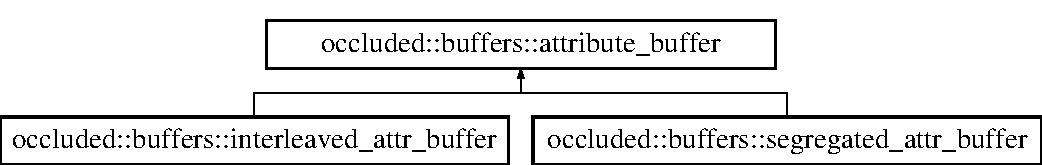
\includegraphics[height=2.000000cm]{classoccluded_1_1buffers_1_1attribute__buffer}
\end{center}
\end{figure}
\subsection*{Public Member Functions}
\begin{DoxyCompactItemize}
\item 
\hyperlink{classoccluded_1_1buffers_1_1attribute__buffer_a7c3a087b1ec1c67ba66e2385050d1139}{attribute\+\_\+buffer} (const \hyperlink{classoccluded_1_1buffers_1_1attributes_1_1attribute__map}{attributes\+::attribute\+\_\+map} \&map)
\begin{DoxyCompactList}\small\item\em Initializes the attribute buffer. \end{DoxyCompactList}\item 
virtual void \hyperlink{classoccluded_1_1buffers_1_1attribute__buffer_a323a2283330b0bcf4909e8d93bfc594a}{insert\+\_\+values} (const std\+::vector$<$ char $>$ \&values)=0
\begin{DoxyCompactList}\small\item\em Inserts values into the attribute buffer. \end{DoxyCompactList}\item 
\hypertarget{classoccluded_1_1buffers_1_1attribute__buffer_a61f67d28a3825be82be1ef54ad7c632d}{void \hyperlink{classoccluded_1_1buffers_1_1attribute__buffer_a61f67d28a3825be82be1ef54ad7c632d}{clear\+\_\+buffer} ()}\label{classoccluded_1_1buffers_1_1attribute__buffer_a61f67d28a3825be82be1ef54ad7c632d}

\begin{DoxyCompactList}\small\item\em Removes all the values from the buffer. \end{DoxyCompactList}\item 
const std\+::size\+\_\+t \hyperlink{classoccluded_1_1buffers_1_1attribute__buffer_a3d5883862c21deda2cea7739ac9ec5b3}{get\+\_\+byte\+\_\+size} () const 
\begin{DoxyCompactList}\small\item\em Gets the size in bytes of the buffer. \end{DoxyCompactList}\item 
const unsigned int \hyperlink{classoccluded_1_1buffers_1_1attribute__buffer_a5f6d890bde1063a6dcf92af1b0bc36ab}{get\+\_\+num\+\_\+values} () const 
\begin{DoxyCompactList}\small\item\em Get the number of values in the buffer. \end{DoxyCompactList}\item 
const std\+::vector$<$ char $>$ \& \hyperlink{classoccluded_1_1buffers_1_1attribute__buffer_a338701d776783b154bb27fc9e8e7c79b}{get\+\_\+all\+\_\+data} () const 
\begin{DoxyCompactList}\small\item\em Gets the data in the attribute buffer. \end{DoxyCompactList}\item 
const \hyperlink{classoccluded_1_1buffers_1_1attributes_1_1attribute__map}{attributes\+::attribute\+\_\+map} \& \hyperlink{classoccluded_1_1buffers_1_1attribute__buffer_a14a2cdb2675135a00d6b7db18ca02b7a}{get\+\_\+attribute\+\_\+map} () const 
\begin{DoxyCompactList}\small\item\em Gets the attribute map of the attribute buffer. \end{DoxyCompactList}\item 
const std\+::vector$<$ unsigned int $>$ \& \hyperlink{classoccluded_1_1buffers_1_1attribute__buffer_a52e537624fad0f1b22cefade12366d88}{get\+\_\+attribute\+\_\+data\+\_\+offsets} () const 
\begin{DoxyCompactList}\small\item\em Gets the offsets of to the values in attribute buffer. \end{DoxyCompactList}\end{DoxyCompactItemize}
\subsection*{Protected Attributes}
\begin{DoxyCompactItemize}
\item 
\hypertarget{classoccluded_1_1buffers_1_1attribute__buffer_a4b0f0972376235e0b6abdc308972d783}{\hyperlink{classoccluded_1_1buffers_1_1attributes_1_1attribute__map}{attributes\+::attribute\+\_\+map} {\bfseries m\+\_\+map}}\label{classoccluded_1_1buffers_1_1attribute__buffer_a4b0f0972376235e0b6abdc308972d783}

\item 
\hypertarget{classoccluded_1_1buffers_1_1attribute__buffer_a6eb7d66fdb8c85469aaa8e473f454dc3}{std\+::vector$<$ char $>$ {\bfseries m\+\_\+data}}\label{classoccluded_1_1buffers_1_1attribute__buffer_a6eb7d66fdb8c85469aaa8e473f454dc3}

\item 
\hypertarget{classoccluded_1_1buffers_1_1attribute__buffer_af15ffb47f059241a61ff6e1dfec12439}{std\+::vector$<$ unsigned int $>$ {\bfseries m\+\_\+buffer\+Pointers}}\label{classoccluded_1_1buffers_1_1attribute__buffer_af15ffb47f059241a61ff6e1dfec12439}

\item 
\hypertarget{classoccluded_1_1buffers_1_1attribute__buffer_acb44ffcc53b7f4e3ebc83bd69791238d}{unsigned int {\bfseries m\+\_\+num\+Values}}\label{classoccluded_1_1buffers_1_1attribute__buffer_acb44ffcc53b7f4e3ebc83bd69791238d}

\item 
\hypertarget{classoccluded_1_1buffers_1_1attribute__buffer_a23f52b63882d1ea6864995672be40577}{bool {\bfseries m\+\_\+pointers\+Set}}\label{classoccluded_1_1buffers_1_1attribute__buffer_a23f52b63882d1ea6864995672be40577}

\end{DoxyCompactItemize}


\subsection{Detailed Description}
Provides contiguous storage for values associated with attributes. 

Provides contiguous storage for values associated with attributes in an attribute map. 

\subsection{Constructor \& Destructor Documentation}
\hypertarget{classoccluded_1_1buffers_1_1attribute__buffer_a7c3a087b1ec1c67ba66e2385050d1139}{\index{occluded\+::buffers\+::attribute\+\_\+buffer@{occluded\+::buffers\+::attribute\+\_\+buffer}!attribute\+\_\+buffer@{attribute\+\_\+buffer}}
\index{attribute\+\_\+buffer@{attribute\+\_\+buffer}!occluded\+::buffers\+::attribute\+\_\+buffer@{occluded\+::buffers\+::attribute\+\_\+buffer}}
\subsubsection[{attribute\+\_\+buffer}]{\setlength{\rightskip}{0pt plus 5cm}occluded\+::buffers\+::attribute\+\_\+buffer\+::attribute\+\_\+buffer (
\begin{DoxyParamCaption}
\item[{const {\bf attributes\+::attribute\+\_\+map} \&}]{map}
\end{DoxyParamCaption}
)}}\label{classoccluded_1_1buffers_1_1attribute__buffer_a7c3a087b1ec1c67ba66e2385050d1139}


Initializes the attribute buffer. 


\begin{DoxyParams}{Parameters}
{\em map} & A reference to an attribute map.\\
\hline
\end{DoxyParams}
Intializes the attribute buffer using the provided attribute map. 

\subsection{Member Function Documentation}
\hypertarget{classoccluded_1_1buffers_1_1attribute__buffer_a338701d776783b154bb27fc9e8e7c79b}{\index{occluded\+::buffers\+::attribute\+\_\+buffer@{occluded\+::buffers\+::attribute\+\_\+buffer}!get\+\_\+all\+\_\+data@{get\+\_\+all\+\_\+data}}
\index{get\+\_\+all\+\_\+data@{get\+\_\+all\+\_\+data}!occluded\+::buffers\+::attribute\+\_\+buffer@{occluded\+::buffers\+::attribute\+\_\+buffer}}
\subsubsection[{get\+\_\+all\+\_\+data}]{\setlength{\rightskip}{0pt plus 5cm}occluded\+::buffers\+::attribute\+\_\+buffer\+::get\+\_\+all\+\_\+data (
\begin{DoxyParamCaption}
{}
\end{DoxyParamCaption}
) const}}\label{classoccluded_1_1buffers_1_1attribute__buffer_a338701d776783b154bb27fc9e8e7c79b}


Gets the data in the attribute buffer. 

\begin{DoxyReturn}{Returns}
A reference to a vector of character representing the values stored in the attribute buffer. 
\end{DoxyReturn}
\hypertarget{classoccluded_1_1buffers_1_1attribute__buffer_a52e537624fad0f1b22cefade12366d88}{\index{occluded\+::buffers\+::attribute\+\_\+buffer@{occluded\+::buffers\+::attribute\+\_\+buffer}!get\+\_\+attribute\+\_\+data\+\_\+offsets@{get\+\_\+attribute\+\_\+data\+\_\+offsets}}
\index{get\+\_\+attribute\+\_\+data\+\_\+offsets@{get\+\_\+attribute\+\_\+data\+\_\+offsets}!occluded\+::buffers\+::attribute\+\_\+buffer@{occluded\+::buffers\+::attribute\+\_\+buffer}}
\subsubsection[{get\+\_\+attribute\+\_\+data\+\_\+offsets}]{\setlength{\rightskip}{0pt plus 5cm}occluded\+::buffers\+::attribute\+\_\+buffer\+::get\+\_\+attribute\+\_\+data\+\_\+offsets (
\begin{DoxyParamCaption}
{}
\end{DoxyParamCaption}
) const}}\label{classoccluded_1_1buffers_1_1attribute__buffer_a52e537624fad0f1b22cefade12366d88}


Gets the offsets of to the values in attribute buffer. 

\begin{DoxyReturn}{Returns}
A reference to a vector of unsigned integers representing the location of the first value of each attribute in the attribute buffer. 
\end{DoxyReturn}
\hypertarget{classoccluded_1_1buffers_1_1attribute__buffer_a14a2cdb2675135a00d6b7db18ca02b7a}{\index{occluded\+::buffers\+::attribute\+\_\+buffer@{occluded\+::buffers\+::attribute\+\_\+buffer}!get\+\_\+attribute\+\_\+map@{get\+\_\+attribute\+\_\+map}}
\index{get\+\_\+attribute\+\_\+map@{get\+\_\+attribute\+\_\+map}!occluded\+::buffers\+::attribute\+\_\+buffer@{occluded\+::buffers\+::attribute\+\_\+buffer}}
\subsubsection[{get\+\_\+attribute\+\_\+map}]{\setlength{\rightskip}{0pt plus 5cm}occluded\+::buffers\+::attribute\+\_\+buffer\+::get\+\_\+attribute\+\_\+map (
\begin{DoxyParamCaption}
{}
\end{DoxyParamCaption}
) const}}\label{classoccluded_1_1buffers_1_1attribute__buffer_a14a2cdb2675135a00d6b7db18ca02b7a}


Gets the attribute map of the attribute buffer. 

\begin{DoxyReturn}{Returns}
A reference to the attribute map of the attribute buffer. 
\end{DoxyReturn}
\hypertarget{classoccluded_1_1buffers_1_1attribute__buffer_a3d5883862c21deda2cea7739ac9ec5b3}{\index{occluded\+::buffers\+::attribute\+\_\+buffer@{occluded\+::buffers\+::attribute\+\_\+buffer}!get\+\_\+byte\+\_\+size@{get\+\_\+byte\+\_\+size}}
\index{get\+\_\+byte\+\_\+size@{get\+\_\+byte\+\_\+size}!occluded\+::buffers\+::attribute\+\_\+buffer@{occluded\+::buffers\+::attribute\+\_\+buffer}}
\subsubsection[{get\+\_\+byte\+\_\+size}]{\setlength{\rightskip}{0pt plus 5cm}occluded\+::buffers\+::attribute\+\_\+buffer\+::get\+\_\+byte\+\_\+size (
\begin{DoxyParamCaption}
{}
\end{DoxyParamCaption}
) const}}\label{classoccluded_1_1buffers_1_1attribute__buffer_a3d5883862c21deda2cea7739ac9ec5b3}


Gets the size in bytes of the buffer. 

\begin{DoxyReturn}{Returns}
A std\+::size\+\_\+t representing the size of the attribute buffer in bytes. 
\end{DoxyReturn}
\hypertarget{classoccluded_1_1buffers_1_1attribute__buffer_a5f6d890bde1063a6dcf92af1b0bc36ab}{\index{occluded\+::buffers\+::attribute\+\_\+buffer@{occluded\+::buffers\+::attribute\+\_\+buffer}!get\+\_\+num\+\_\+values@{get\+\_\+num\+\_\+values}}
\index{get\+\_\+num\+\_\+values@{get\+\_\+num\+\_\+values}!occluded\+::buffers\+::attribute\+\_\+buffer@{occluded\+::buffers\+::attribute\+\_\+buffer}}
\subsubsection[{get\+\_\+num\+\_\+values}]{\setlength{\rightskip}{0pt plus 5cm}occluded\+::buffers\+::attribute\+\_\+buffer\+::get\+\_\+num\+\_\+values (
\begin{DoxyParamCaption}
{}
\end{DoxyParamCaption}
) const}}\label{classoccluded_1_1buffers_1_1attribute__buffer_a5f6d890bde1063a6dcf92af1b0bc36ab}


Get the number of values in the buffer. 

\begin{DoxyReturn}{Returns}
An unsigned int representing the number of values in the buffer. 
\end{DoxyReturn}
\hypertarget{classoccluded_1_1buffers_1_1attribute__buffer_a323a2283330b0bcf4909e8d93bfc594a}{\index{occluded\+::buffers\+::attribute\+\_\+buffer@{occluded\+::buffers\+::attribute\+\_\+buffer}!insert\+\_\+values@{insert\+\_\+values}}
\index{insert\+\_\+values@{insert\+\_\+values}!occluded\+::buffers\+::attribute\+\_\+buffer@{occluded\+::buffers\+::attribute\+\_\+buffer}}
\subsubsection[{insert\+\_\+values}]{\setlength{\rightskip}{0pt plus 5cm}occluded\+::buffers\+::attribute\+\_\+buffer\+::insert\+\_\+values (
\begin{DoxyParamCaption}
\item[{const std\+::vector$<$ char $>$ \&}]{values}
\end{DoxyParamCaption}
)\hspace{0.3cm}{\ttfamily [pure virtual]}}}\label{classoccluded_1_1buffers_1_1attribute__buffer_a323a2283330b0bcf4909e8d93bfc594a}


Inserts values into the attribute buffer. 


\begin{DoxyParams}{Parameters}
{\em values} & A reference to a vector of characters representing the values to be inserted.\\
\hline
\end{DoxyParams}
Insertes a values into the attribute buffer. The values are inserted such a way that the organization of the values in the buffer is preserved. The values in the vector parameter are assumed to be organized in the same way as the attributes in the attribute map. If inserting a single value, a single value must be inserted for every attribute in the attribute map. 

Implemented in \hyperlink{classoccluded_1_1buffers_1_1interleaved__attr__buffer_a7347f20462c3bb9744602fc159e54e00}{occluded\+::buffers\+::interleaved\+\_\+attr\+\_\+buffer}, and \hyperlink{classoccluded_1_1buffers_1_1segregated__attr__buffer_a437ef88504021dc75d45dff010986128}{occluded\+::buffers\+::segregated\+\_\+attr\+\_\+buffer}.



The documentation for this class was generated from the following files\+:\begin{DoxyCompactItemize}
\item 
Occluded\+Library/buffers/attribute\+\_\+buffer.\+h\item 
Occluded\+Library/buffers/attribute\+\_\+buffer.\+cpp\end{DoxyCompactItemize}

\hypertarget{classoccluded_1_1buffers_1_1attribute__buffer__factory}{\section{occluded\+:\+:buffers\+:\+:attribute\+\_\+buffer\+\_\+factory Class Reference}
\label{classoccluded_1_1buffers_1_1attribute__buffer__factory}\index{occluded\+::buffers\+::attribute\+\_\+buffer\+\_\+factory@{occluded\+::buffers\+::attribute\+\_\+buffer\+\_\+factory}}
}
\subsection*{Static Public Member Functions}
\begin{DoxyCompactItemize}
\item 
\hypertarget{classoccluded_1_1buffers_1_1attribute__buffer__factory_a3bc5d7f71d7264101642207c0c4f102c}{static std\+::auto\+\_\+ptr\\*
$<$ \hyperlink{classoccluded_1_1buffers_1_1attribute__buffer}{attribute\+\_\+buffer} $>$ {\bfseries create\+\_\+attribute\+\_\+buffer} (const \hyperlink{classoccluded_1_1buffers_1_1attributes_1_1attribute__map}{attributes\+::attribute\+\_\+map} \&map)}\label{classoccluded_1_1buffers_1_1attribute__buffer__factory_a3bc5d7f71d7264101642207c0c4f102c}

\end{DoxyCompactItemize}


The documentation for this class was generated from the following files\+:\begin{DoxyCompactItemize}
\item 
Occluded\+Library/buffers/attribute\+\_\+buffer\+\_\+factory.\+h\item 
Occluded\+Library/buffers/attribute\+\_\+buffer\+\_\+factory.\+cpp\end{DoxyCompactItemize}

\hypertarget{classoccluded_1_1buffers_1_1attributes_1_1attribute__map}{\section{occluded\+:\+:buffers\+:\+:attributes\+:\+:attribute\+\_\+map Class Reference}
\label{classoccluded_1_1buffers_1_1attributes_1_1attribute__map}\index{occluded\+::buffers\+::attributes\+::attribute\+\_\+map@{occluded\+::buffers\+::attributes\+::attribute\+\_\+map}}
}
\subsection*{Public Member Functions}
\begin{DoxyCompactItemize}
\item 
\hypertarget{classoccluded_1_1buffers_1_1attributes_1_1attribute__map_a4915c4e6bfd59584dc22fb2685f40d02}{{\bfseries attribute\+\_\+map} (const bool interleaved)}\label{classoccluded_1_1buffers_1_1attributes_1_1attribute__map_a4915c4e6bfd59584dc22fb2685f40d02}

\item 
\hypertarget{classoccluded_1_1buffers_1_1attributes_1_1attribute__map_a23c2b0154dd3478fc1877a04e479624a}{void {\bfseries add\+\_\+attribute} (const \hyperlink{classoccluded_1_1buffers_1_1attributes_1_1attribute}{attribute} \&new\+Attrib)}\label{classoccluded_1_1buffers_1_1attributes_1_1attribute__map_a23c2b0154dd3478fc1877a04e479624a}

\item 
\hypertarget{classoccluded_1_1buffers_1_1attributes_1_1attribute__map_a6c64d6c47c0942c714d0105163e250aa}{void {\bfseries end\+\_\+definition} ()}\label{classoccluded_1_1buffers_1_1attributes_1_1attribute__map_a6c64d6c47c0942c714d0105163e250aa}

\item 
\hypertarget{classoccluded_1_1buffers_1_1attributes_1_1attribute__map_a4b55a620f00eaf746ef55063b8e9f6ff}{void {\bfseries reset} (const bool interleaved)}\label{classoccluded_1_1buffers_1_1attributes_1_1attribute__map_a4b55a620f00eaf746ef55063b8e9f6ff}

\item 
\hypertarget{classoccluded_1_1buffers_1_1attributes_1_1attribute__map_ad886ab232a2f74be15e3930145545caf}{const std\+::size\+\_\+t {\bfseries get\+\_\+byte\+\_\+size} () const }\label{classoccluded_1_1buffers_1_1attributes_1_1attribute__map_ad886ab232a2f74be15e3930145545caf}

\item 
\hypertarget{classoccluded_1_1buffers_1_1attributes_1_1attribute__map_ae78420eeed982caaaa77cada069c315f}{const unsigned int {\bfseries get\+\_\+attrib\+\_\+count} () const }\label{classoccluded_1_1buffers_1_1attributes_1_1attribute__map_ae78420eeed982caaaa77cada069c315f}

\item 
\hypertarget{classoccluded_1_1buffers_1_1attributes_1_1attribute__map_a7c40376c72ad8b85e936213af5abfccf}{const std\+::vector$<$ const \\*
\hyperlink{classoccluded_1_1buffers_1_1attributes_1_1attribute}{attribute} $>$ \& {\bfseries get\+\_\+attributes} () const }\label{classoccluded_1_1buffers_1_1attributes_1_1attribute__map_a7c40376c72ad8b85e936213af5abfccf}

\item 
\hypertarget{classoccluded_1_1buffers_1_1attributes_1_1attribute__map_a378a2e5d7cb0371d45267ef1018f01e0}{const bool {\bfseries is\+\_\+interleaved} () const }\label{classoccluded_1_1buffers_1_1attributes_1_1attribute__map_a378a2e5d7cb0371d45267ef1018f01e0}

\item 
\hypertarget{classoccluded_1_1buffers_1_1attributes_1_1attribute__map_afc2dc57c1bdc2dd5f82a145925243642}{const bool {\bfseries being\+\_\+defined} () const }\label{classoccluded_1_1buffers_1_1attributes_1_1attribute__map_afc2dc57c1bdc2dd5f82a145925243642}

\end{DoxyCompactItemize}


The documentation for this class was generated from the following files\+:\begin{DoxyCompactItemize}
\item 
Occluded\+Library/buffers/attributes/attribute\+\_\+map.\+h\item 
Occluded\+Library/buffers/attributes/attribute\+\_\+map.\+cpp\end{DoxyCompactItemize}

\hypertarget{classoccluded_1_1scene_1_1objects_1_1camera}{\section{occluded\+:\+:scene\+:\+:objects\+:\+:camera Class Reference}
\label{classoccluded_1_1scene_1_1objects_1_1camera}\index{occluded\+::scene\+::objects\+::camera@{occluded\+::scene\+::objects\+::camera}}
}


An abstract class that contains all the methods other camera sub classes must implement.  




{\ttfamily \#include $<$camera.\+h$>$}

Inheritance diagram for occluded\+:\+:scene\+:\+:objects\+:\+:camera\+:\begin{figure}[H]
\begin{center}
\leavevmode
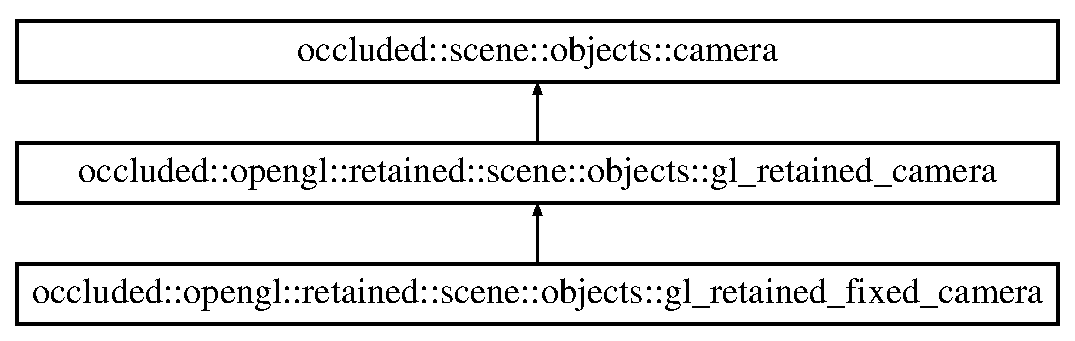
\includegraphics[height=3.000000cm]{classoccluded_1_1scene_1_1objects_1_1camera}
\end{center}
\end{figure}
\subsection*{Public Member Functions}
\begin{DoxyCompactItemize}
\item 
virtual void \hyperlink{classoccluded_1_1scene_1_1objects_1_1camera_a4e62fa6846f1009409a7ed87fe03f8ca}{set\+\_\+for\+\_\+render} () const =0
\begin{DoxyCompactList}\small\item\em Sets this camera to the camera that will be used for rendering. \end{DoxyCompactList}\item 
virtual const \\*
\hyperlink{classoccluded_1_1scene_1_1nodes_1_1transformation}{occluded\+::transformation} \& \hyperlink{classoccluded_1_1scene_1_1objects_1_1camera_ae045f6f1549e58c3211e75a708f8f490}{get\+\_\+projection} () const =0
\begin{DoxyCompactList}\small\item\em Gets the projection transformation. \end{DoxyCompactList}\item 
virtual const \\*
\hyperlink{classoccluded_1_1scene_1_1nodes_1_1transformation}{occluded\+::transformation} \& \hyperlink{classoccluded_1_1scene_1_1objects_1_1camera_aa4168c8ffacdf6a3eb52b528d4780d4e}{get\+\_\+view} () const =0
\begin{DoxyCompactList}\small\item\em Gets the view transformation. \end{DoxyCompactList}\end{DoxyCompactItemize}


\subsection{Detailed Description}
An abstract class that contains all the methods other camera sub classes must implement. 

An abstract class that contains all the methods other camera sub classes must implement. A camera contains all the information necessary for displaying a scene of objects from a specific point of view. It specifies what the view volumes shape is, where that view volume is located, how the the view volume is orientated, and how objects in that view volume are projected onto a 2d surface that the user sees. This usually is implemented by two transformations\+: 1) The view transformation 2) The projection transformation 

\subsection{Member Function Documentation}
\hypertarget{classoccluded_1_1scene_1_1objects_1_1camera_ae045f6f1549e58c3211e75a708f8f490}{\index{occluded\+::scene\+::objects\+::camera@{occluded\+::scene\+::objects\+::camera}!get\+\_\+projection@{get\+\_\+projection}}
\index{get\+\_\+projection@{get\+\_\+projection}!occluded\+::scene\+::objects\+::camera@{occluded\+::scene\+::objects\+::camera}}
\subsubsection[{get\+\_\+projection}]{\setlength{\rightskip}{0pt plus 5cm}occluded\+::scene\+::objects\+::camera\+::get\+\_\+projection (
\begin{DoxyParamCaption}
{}
\end{DoxyParamCaption}
) const\hspace{0.3cm}{\ttfamily [pure virtual]}}}\label{classoccluded_1_1scene_1_1objects_1_1camera_ae045f6f1549e58c3211e75a708f8f490}


Gets the projection transformation. 

\begin{DoxyReturn}{Returns}
A constant reference to the transformation object representing the projection transformation. 
\end{DoxyReturn}


Implemented in \hyperlink{classoccluded_1_1opengl_1_1retained_1_1scene_1_1objects_1_1gl__retained__fixed__camera_a167066c59a31c58a34bf8112e3f9ef37}{occluded\+::opengl\+::retained\+::scene\+::objects\+::gl\+\_\+retained\+\_\+fixed\+\_\+camera}.

\hypertarget{classoccluded_1_1scene_1_1objects_1_1camera_aa4168c8ffacdf6a3eb52b528d4780d4e}{\index{occluded\+::scene\+::objects\+::camera@{occluded\+::scene\+::objects\+::camera}!get\+\_\+view@{get\+\_\+view}}
\index{get\+\_\+view@{get\+\_\+view}!occluded\+::scene\+::objects\+::camera@{occluded\+::scene\+::objects\+::camera}}
\subsubsection[{get\+\_\+view}]{\setlength{\rightskip}{0pt plus 5cm}occluded\+::scene\+::objects\+::camera\+::get\+\_\+view (
\begin{DoxyParamCaption}
{}
\end{DoxyParamCaption}
) const\hspace{0.3cm}{\ttfamily [pure virtual]}}}\label{classoccluded_1_1scene_1_1objects_1_1camera_aa4168c8ffacdf6a3eb52b528d4780d4e}


Gets the view transformation. 

\begin{DoxyReturn}{Returns}
A constant reference to the transformation object containing the view transformation. 
\end{DoxyReturn}


Implemented in \hyperlink{classoccluded_1_1opengl_1_1retained_1_1scene_1_1objects_1_1gl__retained__fixed__camera_a354c288a4f0c6d05bcbbb256d7c65931}{occluded\+::opengl\+::retained\+::scene\+::objects\+::gl\+\_\+retained\+\_\+fixed\+\_\+camera}.

\hypertarget{classoccluded_1_1scene_1_1objects_1_1camera_a4e62fa6846f1009409a7ed87fe03f8ca}{\index{occluded\+::scene\+::objects\+::camera@{occluded\+::scene\+::objects\+::camera}!set\+\_\+for\+\_\+render@{set\+\_\+for\+\_\+render}}
\index{set\+\_\+for\+\_\+render@{set\+\_\+for\+\_\+render}!occluded\+::scene\+::objects\+::camera@{occluded\+::scene\+::objects\+::camera}}
\subsubsection[{set\+\_\+for\+\_\+render}]{\setlength{\rightskip}{0pt plus 5cm}occluded\+::scene\+::objects\+::camera\+::set\+\_\+for\+\_\+render (
\begin{DoxyParamCaption}
{}
\end{DoxyParamCaption}
) const\hspace{0.3cm}{\ttfamily [pure virtual]}}}\label{classoccluded_1_1scene_1_1objects_1_1camera_a4e62fa6846f1009409a7ed87fe03f8ca}


Sets this camera to the camera that will be used for rendering. 

Sets this camera as the camera to be used for next render. 

Implemented in \hyperlink{classoccluded_1_1opengl_1_1retained_1_1scene_1_1objects_1_1gl__retained__fixed__camera_a81ea1cd723428ac234ca814c43363a90}{occluded\+::opengl\+::retained\+::scene\+::objects\+::gl\+\_\+retained\+\_\+fixed\+\_\+camera}.



The documentation for this class was generated from the following file\+:\begin{DoxyCompactItemize}
\item 
Occluded\+Library/scene/objects/camera.\+h\end{DoxyCompactItemize}

\hypertarget{classoccluded_1_1utilities_1_1files_1_1file__reader}{\section{occluded\+:\+:utilities\+:\+:files\+:\+:file\+\_\+reader Class Reference}
\label{classoccluded_1_1utilities_1_1files_1_1file__reader}\index{occluded\+::utilities\+::files\+::file\+\_\+reader@{occluded\+::utilities\+::files\+::file\+\_\+reader}}
}


A class that provides ways of reading files.  




{\ttfamily \#include $<$file\+\_\+reader.\+h$>$}

\subsection*{Static Public Member Functions}
\begin{DoxyCompactItemize}
\item 
static const std\+::string \hyperlink{classoccluded_1_1utilities_1_1files_1_1file__reader_a905fd62c6bc5da558c3c303c4a5fe40a}{get\+\_\+string\+\_\+from\+\_\+file} (const std\+::string \&file\+Path)
\begin{DoxyCompactList}\small\item\em Reads a file's contents into a string. \end{DoxyCompactList}\end{DoxyCompactItemize}


\subsection{Detailed Description}
A class that provides ways of reading files. 

A utility class that provides ways of reading files for processing in the occluded library. 

\subsection{Member Function Documentation}
\hypertarget{classoccluded_1_1utilities_1_1files_1_1file__reader_a905fd62c6bc5da558c3c303c4a5fe40a}{\index{occluded\+::utilities\+::files\+::file\+\_\+reader@{occluded\+::utilities\+::files\+::file\+\_\+reader}!get\+\_\+string\+\_\+from\+\_\+file@{get\+\_\+string\+\_\+from\+\_\+file}}
\index{get\+\_\+string\+\_\+from\+\_\+file@{get\+\_\+string\+\_\+from\+\_\+file}!occluded\+::utilities\+::files\+::file\+\_\+reader@{occluded\+::utilities\+::files\+::file\+\_\+reader}}
\subsubsection[{get\+\_\+string\+\_\+from\+\_\+file}]{\setlength{\rightskip}{0pt plus 5cm}occluded\+::utilities\+::files\+::file\+\_\+reader\+::get\+\_\+string\+\_\+from\+\_\+file (
\begin{DoxyParamCaption}
\item[{const std\+::string \&}]{file\+Path}
\end{DoxyParamCaption}
)\hspace{0.3cm}{\ttfamily [static]}}}\label{classoccluded_1_1utilities_1_1files_1_1file__reader_a905fd62c6bc5da558c3c303c4a5fe40a}


Reads a file's contents into a string. 


\begin{DoxyParams}{Parameters}
{\em file\+Path} & A reference to a string representing the file path of the file. \\
\hline
\end{DoxyParams}
\begin{DoxyReturn}{Returns}
A string containing the contents of the file.
\end{DoxyReturn}
Reads the contents of the file located at the file\+Path into a string preserving new line characters. 

The documentation for this class was generated from the following files\+:\begin{DoxyCompactItemize}
\item 
Occluded\+Library/utilities/files/file\+\_\+reader.\+h\item 
Occluded\+Library/utilities/files/file\+\_\+reader.\+cpp\end{DoxyCompactItemize}

\hypertarget{classoccluded_1_1opengl_1_1retained_1_1gl__attribute__buffer}{\section{occluded\+:\+:opengl\+:\+:retained\+:\+:gl\+\_\+attribute\+\_\+buffer Class Reference}
\label{classoccluded_1_1opengl_1_1retained_1_1gl__attribute__buffer}\index{occluded\+::opengl\+::retained\+::gl\+\_\+attribute\+\_\+buffer@{occluded\+::opengl\+::retained\+::gl\+\_\+attribute\+\_\+buffer}}
}


A wrapper class for an Open\+G\+L buffer.  




{\ttfamily \#include $<$gl\+\_\+attribute\+\_\+buffer.\+h$>$}

\subsection*{Public Member Functions}
\begin{DoxyCompactItemize}
\item 
\hyperlink{classoccluded_1_1opengl_1_1retained_1_1gl__attribute__buffer_a22cdc11d70684a364895715b12293487}{gl\+\_\+attribute\+\_\+buffer} (const \hyperlink{classoccluded_1_1buffers_1_1attributes_1_1attribute__map}{buffers\+::attributes\+::attribute\+\_\+map} \&map, const \hyperlink{classoccluded_1_1opengl_1_1retained_1_1shaders_1_1shader__program}{shaders\+::shader\+\_\+program} \&shader\+Prog, const buffer\+\_\+usage\+\_\+t usage)
\begin{DoxyCompactList}\small\item\em Initialize the buffer. \end{DoxyCompactList}\item 
void \hyperlink{classoccluded_1_1opengl_1_1retained_1_1gl__attribute__buffer_afd58deefb5659c0cd9a316263515b68f}{insert\+\_\+values} (const std\+::vector$<$ char $>$ \&values)
\begin{DoxyCompactList}\small\item\em Inserts data into the buffer. \end{DoxyCompactList}\item 
void \hyperlink{classoccluded_1_1opengl_1_1retained_1_1gl__attribute__buffer_a0bc941bf7603a80ea249cd1d64cc2b67}{bind\+\_\+buffer} () const 
\begin{DoxyCompactList}\small\item\em Binds the buffer as an array buffer object. \end{DoxyCompactList}\item 
const G\+Luint \hyperlink{classoccluded_1_1opengl_1_1retained_1_1gl__attribute__buffer_ab23624ebadcabdcb0d028e2fe0039ffd}{get\+\_\+id} () const 
\begin{DoxyCompactList}\small\item\em Gets the id of the Open\+G\+L buffer object. \end{DoxyCompactList}\item 
const \\*
\hyperlink{classoccluded_1_1buffers_1_1attributes_1_1attribute__map}{buffers\+::attributes\+::attribute\+\_\+map} \& \hyperlink{classoccluded_1_1opengl_1_1retained_1_1gl__attribute__buffer_a1241841aa913b0df057b5d885f1447b4}{get\+\_\+buffer\+\_\+map} () const 
\begin{DoxyCompactList}\small\item\em Gets the attribute\+\_\+map of the attribute\+\_\+buffer. \end{DoxyCompactList}\item 
void \hyperlink{classoccluded_1_1opengl_1_1retained_1_1gl__attribute__buffer_ab7707122e284ee1c28bf238885ae6a59}{prepare\+\_\+for\+\_\+render} () const 
\begin{DoxyCompactList}\small\item\em Sets up the buffer for rendering. \end{DoxyCompactList}\end{DoxyCompactItemize}


\subsection{Detailed Description}
A wrapper class for an Open\+G\+L buffer. 

A wrapper class for an Open\+G\+L buffer object. It stores information about the buffer to allow for quickly accessing that information without querying the Open\+G\+L buffer object. It also contains an attribute\+\_\+buffer object that will allow for storage of data outside of Open\+G\+L which makes inserting data into the buffer significantly more easy as well as allowing for checking to make sure data being inserted is valid. 

\subsection{Constructor \& Destructor Documentation}
\hypertarget{classoccluded_1_1opengl_1_1retained_1_1gl__attribute__buffer_a22cdc11d70684a364895715b12293487}{\index{occluded\+::opengl\+::retained\+::gl\+\_\+attribute\+\_\+buffer@{occluded\+::opengl\+::retained\+::gl\+\_\+attribute\+\_\+buffer}!gl\+\_\+attribute\+\_\+buffer@{gl\+\_\+attribute\+\_\+buffer}}
\index{gl\+\_\+attribute\+\_\+buffer@{gl\+\_\+attribute\+\_\+buffer}!occluded\+::opengl\+::retained\+::gl\+\_\+attribute\+\_\+buffer@{occluded\+::opengl\+::retained\+::gl\+\_\+attribute\+\_\+buffer}}
\subsubsection[{gl\+\_\+attribute\+\_\+buffer}]{\setlength{\rightskip}{0pt plus 5cm}occluded\+::opengl\+::retained\+::gl\+\_\+attribute\+\_\+buffer\+::gl\+\_\+attribute\+\_\+buffer (
\begin{DoxyParamCaption}
\item[{const {\bf buffers\+::attributes\+::attribute\+\_\+map} \&}]{map, }
\item[{const {\bf shaders\+::shader\+\_\+program} \&}]{shader\+Prog, }
\item[{const buffer\+\_\+usage\+\_\+t}]{usage}
\end{DoxyParamCaption}
)}}\label{classoccluded_1_1opengl_1_1retained_1_1gl__attribute__buffer_a22cdc11d70684a364895715b12293487}


Initialize the buffer. 


\begin{DoxyParams}{Parameters}
{\em map} & A reference to an attribute map. \\
\hline
{\em shader\+Prog} & A reference to a shader program. \\
\hline
{\em usage} & A enumerable that will be used to tell Open\+G\+L how the buffer will be used.\\
\hline
\end{DoxyParams}
Generate the an Open\+G\+L buffer object, creates an attribute buffer to store data inserted into the buffer, and binds that buffer as an array buffer. 

\subsection{Member Function Documentation}
\hypertarget{classoccluded_1_1opengl_1_1retained_1_1gl__attribute__buffer_a0bc941bf7603a80ea249cd1d64cc2b67}{\index{occluded\+::opengl\+::retained\+::gl\+\_\+attribute\+\_\+buffer@{occluded\+::opengl\+::retained\+::gl\+\_\+attribute\+\_\+buffer}!bind\+\_\+buffer@{bind\+\_\+buffer}}
\index{bind\+\_\+buffer@{bind\+\_\+buffer}!occluded\+::opengl\+::retained\+::gl\+\_\+attribute\+\_\+buffer@{occluded\+::opengl\+::retained\+::gl\+\_\+attribute\+\_\+buffer}}
\subsubsection[{bind\+\_\+buffer}]{\setlength{\rightskip}{0pt plus 5cm}occluded\+::opengl\+::retained\+::gl\+\_\+attribute\+\_\+buffer\+::bind\+\_\+buffer (
\begin{DoxyParamCaption}
{}
\end{DoxyParamCaption}
) const}}\label{classoccluded_1_1opengl_1_1retained_1_1gl__attribute__buffer_a0bc941bf7603a80ea249cd1d64cc2b67}


Binds the buffer as an array buffer object. 

Binds the buffer as an array buffer object and sets the Open\+G\+L buffer's data store to the contents of the attribute buffer. Should be called prior to using the buffer in an Open\+G\+L draw call or after the data in the attribute buffer has changed. \hypertarget{classoccluded_1_1opengl_1_1retained_1_1gl__attribute__buffer_a1241841aa913b0df057b5d885f1447b4}{\index{occluded\+::opengl\+::retained\+::gl\+\_\+attribute\+\_\+buffer@{occluded\+::opengl\+::retained\+::gl\+\_\+attribute\+\_\+buffer}!get\+\_\+buffer\+\_\+map@{get\+\_\+buffer\+\_\+map}}
\index{get\+\_\+buffer\+\_\+map@{get\+\_\+buffer\+\_\+map}!occluded\+::opengl\+::retained\+::gl\+\_\+attribute\+\_\+buffer@{occluded\+::opengl\+::retained\+::gl\+\_\+attribute\+\_\+buffer}}
\subsubsection[{get\+\_\+buffer\+\_\+map}]{\setlength{\rightskip}{0pt plus 5cm}occluded\+::opengl\+::retained\+::gl\+\_\+attribute\+\_\+buffer\+::get\+\_\+buffer\+\_\+map (
\begin{DoxyParamCaption}
{}
\end{DoxyParamCaption}
) const}}\label{classoccluded_1_1opengl_1_1retained_1_1gl__attribute__buffer_a1241841aa913b0df057b5d885f1447b4}


Gets the attribute\+\_\+map of the attribute\+\_\+buffer. 

\begin{DoxyReturn}{Returns}
A reference to the attribute\+\_\+map used in the attribute\+\_\+buffer contained by the \hyperlink{classoccluded_1_1opengl_1_1retained_1_1gl__attribute__buffer}{gl\+\_\+attribute\+\_\+buffer}.
\end{DoxyReturn}
Gets a reference to the attribute\+\_\+map used by the attribute\+\_\+buffer contained by the \hyperlink{classoccluded_1_1opengl_1_1retained_1_1gl__attribute__buffer}{gl\+\_\+attribute\+\_\+buffer}. Intended to be used for formatting data to be inserted into the \hyperlink{classoccluded_1_1opengl_1_1retained_1_1gl__attribute__buffer}{gl\+\_\+attribute\+\_\+buffer} as well as determining the inputs to a gl\+Vertex\+Attrib\+Pointer call. \hypertarget{classoccluded_1_1opengl_1_1retained_1_1gl__attribute__buffer_ab23624ebadcabdcb0d028e2fe0039ffd}{\index{occluded\+::opengl\+::retained\+::gl\+\_\+attribute\+\_\+buffer@{occluded\+::opengl\+::retained\+::gl\+\_\+attribute\+\_\+buffer}!get\+\_\+id@{get\+\_\+id}}
\index{get\+\_\+id@{get\+\_\+id}!occluded\+::opengl\+::retained\+::gl\+\_\+attribute\+\_\+buffer@{occluded\+::opengl\+::retained\+::gl\+\_\+attribute\+\_\+buffer}}
\subsubsection[{get\+\_\+id}]{\setlength{\rightskip}{0pt plus 5cm}occluded\+::opengl\+::retained\+::gl\+\_\+attribute\+\_\+buffer\+::get\+\_\+id (
\begin{DoxyParamCaption}
{}
\end{DoxyParamCaption}
) const}}\label{classoccluded_1_1opengl_1_1retained_1_1gl__attribute__buffer_ab23624ebadcabdcb0d028e2fe0039ffd}


Gets the id of the Open\+G\+L buffer object. 

Gets the id of the Open\+G\+L buffer object connected to this buffer. If this buffer is being used in a S\+T\+L container, the value returned will change when the \hyperlink{classoccluded_1_1opengl_1_1retained_1_1gl__attribute__buffer}{gl\+\_\+attribute\+\_\+buffer} is inserted into the container. \begin{DoxyWarning}{Warning}
Do not call gl\+Delete\+Buffer on the id returned from this function call. It will cause an Open\+G\+L to enter an error state when the the gl\+\_\+attribute\+\_\+buffers destructor is called. 
\end{DoxyWarning}
\hypertarget{classoccluded_1_1opengl_1_1retained_1_1gl__attribute__buffer_afd58deefb5659c0cd9a316263515b68f}{\index{occluded\+::opengl\+::retained\+::gl\+\_\+attribute\+\_\+buffer@{occluded\+::opengl\+::retained\+::gl\+\_\+attribute\+\_\+buffer}!insert\+\_\+values@{insert\+\_\+values}}
\index{insert\+\_\+values@{insert\+\_\+values}!occluded\+::opengl\+::retained\+::gl\+\_\+attribute\+\_\+buffer@{occluded\+::opengl\+::retained\+::gl\+\_\+attribute\+\_\+buffer}}
\subsubsection[{insert\+\_\+values}]{\setlength{\rightskip}{0pt plus 5cm}occluded\+::opengl\+::retained\+::gl\+\_\+attribute\+\_\+buffer\+::insert\+\_\+values (
\begin{DoxyParamCaption}
\item[{const std\+::vector$<$ char $>$ \&}]{values}
\end{DoxyParamCaption}
)}}\label{classoccluded_1_1opengl_1_1retained_1_1gl__attribute__buffer_afd58deefb5659c0cd9a316263515b68f}


Inserts data into the buffer. 


\begin{DoxyParams}{Parameters}
{\em A} & reference to a vector of bytes containing the data to be inserted.\\
\hline
\end{DoxyParams}
Inserts data into the attribute buffer, then binds the buffer and sets the Open\+G\+L data store to the data in the attribute buffer for the Open\+G\+L buffer object connected to this buffer. \hypertarget{classoccluded_1_1opengl_1_1retained_1_1gl__attribute__buffer_ab7707122e284ee1c28bf238885ae6a59}{\index{occluded\+::opengl\+::retained\+::gl\+\_\+attribute\+\_\+buffer@{occluded\+::opengl\+::retained\+::gl\+\_\+attribute\+\_\+buffer}!prepare\+\_\+for\+\_\+render@{prepare\+\_\+for\+\_\+render}}
\index{prepare\+\_\+for\+\_\+render@{prepare\+\_\+for\+\_\+render}!occluded\+::opengl\+::retained\+::gl\+\_\+attribute\+\_\+buffer@{occluded\+::opengl\+::retained\+::gl\+\_\+attribute\+\_\+buffer}}
\subsubsection[{prepare\+\_\+for\+\_\+render}]{\setlength{\rightskip}{0pt plus 5cm}occluded\+::opengl\+::retained\+::gl\+\_\+attribute\+\_\+buffer\+::prepare\+\_\+for\+\_\+render (
\begin{DoxyParamCaption}
{}
\end{DoxyParamCaption}
) const}}\label{classoccluded_1_1opengl_1_1retained_1_1gl__attribute__buffer_ab7707122e284ee1c28bf238885ae6a59}


Sets up the buffer for rendering. 

Sets up the buffer for rendering by binding the buffer and setting up the vertex attribute pointers so that the data can be passed to the shader program. Used for making so that a single call can be made prior to a gl\+Draw call. 

The documentation for this class was generated from the following files\+:\begin{DoxyCompactItemize}
\item 
Occluded\+Library/opengl/retained/gl\+\_\+attribute\+\_\+buffer.\+h\item 
Occluded\+Library/opengl/retained/gl\+\_\+attribute\+\_\+buffer.\+cpp\end{DoxyCompactItemize}

\hypertarget{classoccluded_1_1opengl_1_1retained_1_1gl__retained__mesh}{\section{occluded\+:\+:opengl\+:\+:retained\+:\+:gl\+\_\+retained\+\_\+mesh Class Reference}
\label{classoccluded_1_1opengl_1_1retained_1_1gl__retained__mesh}\index{occluded\+::opengl\+::retained\+::gl\+\_\+retained\+\_\+mesh@{occluded\+::opengl\+::retained\+::gl\+\_\+retained\+\_\+mesh}}
}


A mesh implementation for Open\+G\+L retained mode.  




{\ttfamily \#include $<$gl\+\_\+retained\+\_\+mesh.\+h$>$}

Inheritance diagram for occluded\+:\+:opengl\+:\+:retained\+:\+:gl\+\_\+retained\+\_\+mesh\+:\begin{figure}[H]
\begin{center}
\leavevmode
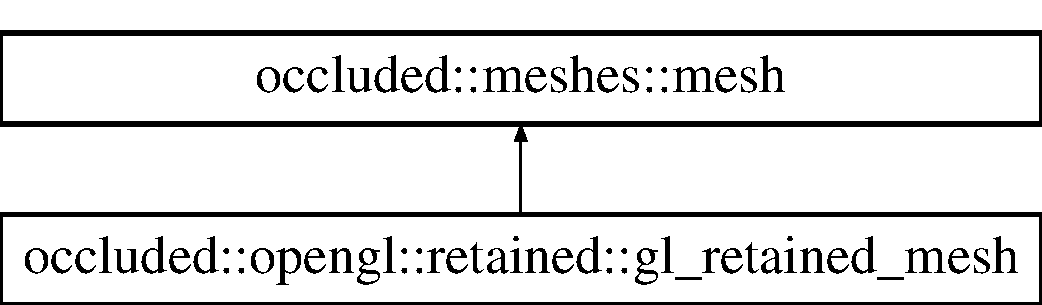
\includegraphics[height=2.000000cm]{classoccluded_1_1opengl_1_1retained_1_1gl__retained__mesh}
\end{center}
\end{figure}
\subsection*{Public Member Functions}
\begin{DoxyCompactItemize}
\item 
\hyperlink{classoccluded_1_1opengl_1_1retained_1_1gl__retained__mesh_a64b7a4795fc93fc81308e1a464debd24}{gl\+\_\+retained\+\_\+mesh} (const G\+Luint vao\+Id, const \hyperlink{classoccluded_1_1buffers_1_1attributes_1_1attribute__map}{occluded\+::buffers\+::attributes\+::attribute\+\_\+map} \&map, const \hyperlink{classoccluded_1_1opengl_1_1retained_1_1shaders_1_1shader__program}{shaders\+::shader\+\_\+program} \&shader\+Prog, const buffer\+\_\+usage\+\_\+t usage=static\+\_\+draw\+\_\+usage, const primitive\+\_\+type\+\_\+t primitive\+Type=primitive\+\_\+triangles)
\begin{DoxyCompactList}\small\item\em Initializes an empty mesh. \end{DoxyCompactList}\item 
\hyperlink{classoccluded_1_1opengl_1_1retained_1_1gl__retained__mesh_ac7b08ac856c790d12581f8ce27be96bf}{gl\+\_\+retained\+\_\+mesh} (const G\+Luint vao\+Id, const \hyperlink{classoccluded_1_1opengl_1_1retained_1_1shaders_1_1shader__program}{shaders\+::shader\+\_\+program} \&shader\+Prog, \hyperlink{classoccluded_1_1opengl_1_1retained_1_1gl__attribute__buffer}{gl\+\_\+attribute\+\_\+buffer} \&buffer, const std\+::vector$<$ unsigned int $>$ \&faces, const primitive\+\_\+type\+\_\+t primitive\+Type=primitive\+\_\+triangles)
\begin{DoxyCompactList}\small\item\em Initializes an mesh. \end{DoxyCompactList}\item 
void \hyperlink{classoccluded_1_1opengl_1_1retained_1_1gl__retained__mesh_aa2018120d3a1dcca990e85a24efe20fb}{draw} () const 
\begin{DoxyCompactList}\small\item\em Draws the mesh. \end{DoxyCompactList}\item 
const std\+::vector$<$ unsigned int $>$ \hyperlink{classoccluded_1_1opengl_1_1retained_1_1gl__retained__mesh_af1df11c76aefccc2bd9b67f839bfcbb8}{add\+\_\+vertices} (const std\+::vector$<$ char $>$ \&vertices)
\begin{DoxyCompactList}\small\item\em Adds vertices to the mesh. \end{DoxyCompactList}\item 
const std\+::vector$<$ unsigned int $>$ \hyperlink{classoccluded_1_1opengl_1_1retained_1_1gl__retained__mesh_a3f0f0574b87516c2a88d1bf14089c801}{add\+\_\+faces} (const std\+::vector$<$ unsigned int $>$ \&face\+Indices)
\begin{DoxyCompactList}\small\item\em Adds faces to the mesh. \end{DoxyCompactList}\item 
const unsigned int \hyperlink{classoccluded_1_1opengl_1_1retained_1_1gl__retained__mesh_ae9f8c756698b09458d61aba3a616f78b}{add\+\_\+face} (const std\+::vector$<$ unsigned int $>$ \&face\+Indcies)
\begin{DoxyCompactList}\small\item\em Adds a single face to the mesh. \end{DoxyCompactList}\item 
const unsigned int \hyperlink{classoccluded_1_1opengl_1_1retained_1_1gl__retained__mesh_a57bfbb414bd06bab36f09c19bc0a4e13}{get\+\_\+num\+\_\+faces} () const 
\begin{DoxyCompactList}\small\item\em Gets the number of faces in the mesh. \end{DoxyCompactList}\item 
const unsigned int \hyperlink{classoccluded_1_1opengl_1_1retained_1_1gl__retained__mesh_ab3efafd282bb6f844bd21ca911cfe9dd}{num\+\_\+verts\+\_\+for\+\_\+next\+\_\+face} (const unsigned int num\+Faces) const 
\begin{DoxyCompactList}\small\item\em Gets the number of vertices needed for the next face. \end{DoxyCompactList}\end{DoxyCompactItemize}


\subsection{Detailed Description}
A mesh implementation for Open\+G\+L retained mode. 

A mesh implementation for Open\+G\+L retained mode. This contains a \hyperlink{classoccluded_1_1opengl_1_1retained_1_1gl__attribute__buffer}{gl\+\_\+attribute\+\_\+buffer} and a vector of unsigned int representing the faces of the of the mesh. This is class contains everything needed to draw a single object in object coordinates. The purpose of this class is to be contained within a model class and allow the model class to render the mesh with a single call. /see \{ \hyperlink{classoccluded_1_1opengl_1_1retained_1_1gl__attribute__buffer}{occluded\+::opengl\+::retained\+::gl\+\_\+attribute\+\_\+buffer} \} 

\subsection{Constructor \& Destructor Documentation}
\hypertarget{classoccluded_1_1opengl_1_1retained_1_1gl__retained__mesh_a64b7a4795fc93fc81308e1a464debd24}{\index{occluded\+::opengl\+::retained\+::gl\+\_\+retained\+\_\+mesh@{occluded\+::opengl\+::retained\+::gl\+\_\+retained\+\_\+mesh}!gl\+\_\+retained\+\_\+mesh@{gl\+\_\+retained\+\_\+mesh}}
\index{gl\+\_\+retained\+\_\+mesh@{gl\+\_\+retained\+\_\+mesh}!occluded\+::opengl\+::retained\+::gl\+\_\+retained\+\_\+mesh@{occluded\+::opengl\+::retained\+::gl\+\_\+retained\+\_\+mesh}}
\subsubsection[{gl\+\_\+retained\+\_\+mesh}]{\setlength{\rightskip}{0pt plus 5cm}occluded\+::opengl\+::retained\+::gl\+\_\+retained\+\_\+mesh\+::gl\+\_\+retained\+\_\+mesh (
\begin{DoxyParamCaption}
\item[{const G\+Luint}]{vao\+Id, }
\item[{const {\bf occluded\+::buffers\+::attributes\+::attribute\+\_\+map} \&}]{map, }
\item[{const {\bf shaders\+::shader\+\_\+program} \&}]{shader\+Prog, }
\item[{const buffer\+\_\+usage\+\_\+t}]{usage = {\ttfamily static\+\_\+draw\+\_\+usage}, }
\item[{const primitive\+\_\+type\+\_\+t}]{primitive\+Type = {\ttfamily primitive\+\_\+triangles}}
\end{DoxyParamCaption}
)}}\label{classoccluded_1_1opengl_1_1retained_1_1gl__retained__mesh_a64b7a4795fc93fc81308e1a464debd24}


Initializes an empty mesh. 


\begin{DoxyParams}{Parameters}
{\em vao\+Id} & A constant G\+Luint that represents the id of an Open\+G\+L vertex attribute object \\
\hline
{\em map} & A reference to the attribute map that will be used to store vertex data. \\
\hline
{\em shader\+Prog} & A refernce to a shader program that will be used to render the mesh. \\
\hline
{\em usage} & A buffer usage type that specifies how the vertex and index data will be used. \\
\hline
{\em primitive\+Type} & A primitive type that specifies which Open\+G\+L primitive will be used to construct the faces of the mesh.\\
\hline
\end{DoxyParams}
Initializes the mesh by constructing an \hyperlink{classoccluded_1_1opengl_1_1retained_1_1gl__attribute__buffer}{gl\+\_\+attribute\+\_\+buffer} from the map, shader program and usage parameters. The default primitive used for constructing the mesh is primitive\+\_\+triangles. This constructor is to be used if the mesh is to be built up from scratch. An exception will be thrown in the attribute map is still being defined or if the shader program has not been linked. \hypertarget{classoccluded_1_1opengl_1_1retained_1_1gl__retained__mesh_ac7b08ac856c790d12581f8ce27be96bf}{\index{occluded\+::opengl\+::retained\+::gl\+\_\+retained\+\_\+mesh@{occluded\+::opengl\+::retained\+::gl\+\_\+retained\+\_\+mesh}!gl\+\_\+retained\+\_\+mesh@{gl\+\_\+retained\+\_\+mesh}}
\index{gl\+\_\+retained\+\_\+mesh@{gl\+\_\+retained\+\_\+mesh}!occluded\+::opengl\+::retained\+::gl\+\_\+retained\+\_\+mesh@{occluded\+::opengl\+::retained\+::gl\+\_\+retained\+\_\+mesh}}
\subsubsection[{gl\+\_\+retained\+\_\+mesh}]{\setlength{\rightskip}{0pt plus 5cm}occluded\+::opengl\+::retained\+::gl\+\_\+retained\+\_\+mesh\+::gl\+\_\+retained\+\_\+mesh (
\begin{DoxyParamCaption}
\item[{const G\+Luint}]{vao\+Id, }
\item[{const {\bf shaders\+::shader\+\_\+program} \&}]{shader\+Prog, }
\item[{{\bf gl\+\_\+attribute\+\_\+buffer} \&}]{buffer, }
\item[{const std\+::vector$<$ unsigned int $>$ \&}]{faces, }
\item[{const primitive\+\_\+type\+\_\+t}]{primitive\+Type = {\ttfamily primitive\+\_\+triangles}}
\end{DoxyParamCaption}
)}}\label{classoccluded_1_1opengl_1_1retained_1_1gl__retained__mesh_ac7b08ac856c790d12581f8ce27be96bf}


Initializes an mesh. 


\begin{DoxyParams}{Parameters}
{\em vao\+Id} & A constant G\+Luint that represents the if of an Open\+G\+L vertex attribute object. \\
\hline
{\em shader\+Prog} & A reference to a shader program that will be used to render the mesh. \\
\hline
{\em buffer} & A reference to a \hyperlink{classoccluded_1_1opengl_1_1retained_1_1gl__attribute__buffer}{gl\+\_\+attribute\+\_\+buffer} which stores the vertice data. \\
\hline
{\em faces} & A reference to a vector of unsigned integers representing the vertices that make up the faces of the mesh. \\
\hline
{\em primitive\+Type} & A primitive type that specifies which Open\+G\+L primitive will be used to construct the faces of the mesh.\\
\hline
\end{DoxyParams}
Initializes the mesh by making a copy of an \hyperlink{classoccluded_1_1opengl_1_1retained_1_1gl__attribute__buffer}{gl\+\_\+attribute\+\_\+buffer} and a vector of indices. he default primitive used for constructing the mesh is primitive\+\_\+triangles. This constructor is to be used if the mesh is to be pre-\/built or to be built up from another mesh. An exception will be thrown in the attribute map is still being defined or if the shader program has not been linked. 

\subsection{Member Function Documentation}
\hypertarget{classoccluded_1_1opengl_1_1retained_1_1gl__retained__mesh_ae9f8c756698b09458d61aba3a616f78b}{\index{occluded\+::opengl\+::retained\+::gl\+\_\+retained\+\_\+mesh@{occluded\+::opengl\+::retained\+::gl\+\_\+retained\+\_\+mesh}!add\+\_\+face@{add\+\_\+face}}
\index{add\+\_\+face@{add\+\_\+face}!occluded\+::opengl\+::retained\+::gl\+\_\+retained\+\_\+mesh@{occluded\+::opengl\+::retained\+::gl\+\_\+retained\+\_\+mesh}}
\subsubsection[{add\+\_\+face}]{\setlength{\rightskip}{0pt plus 5cm}occluded\+::opengl\+::retained\+::gl\+\_\+retained\+\_\+mesh\+::add\+\_\+face (
\begin{DoxyParamCaption}
\item[{const std\+::vector$<$ unsigned int $>$ \&}]{face\+Indcies}
\end{DoxyParamCaption}
)\hspace{0.3cm}{\ttfamily [virtual]}}}\label{classoccluded_1_1opengl_1_1retained_1_1gl__retained__mesh_ae9f8c756698b09458d61aba3a616f78b}


Adds a single face to the mesh. 


\begin{DoxyParams}{Parameters}
{\em face\+Indices} & A reference to a vector of unsigned ints containing the indices of the vertices that make up the face to be added. \\
\hline
\end{DoxyParams}
\begin{DoxyReturn}{Returns}
A unsigned int representing the index of the face that was added.
\end{DoxyReturn}
Adds a face to the mesh that is made up of the vertices specified by the indices in the face\+Indices vector. An exception is thrown if the face\+Indices vector does not contain the correct number of vertices or if it contains a index that does not correspond to a vertex in the the mesh. 

Implements \hyperlink{classoccluded_1_1meshes_1_1mesh_a4be1ad0c1b5144faa4f0e9a9c1d3023b}{occluded\+::meshes\+::mesh}.

\hypertarget{classoccluded_1_1opengl_1_1retained_1_1gl__retained__mesh_a3f0f0574b87516c2a88d1bf14089c801}{\index{occluded\+::opengl\+::retained\+::gl\+\_\+retained\+\_\+mesh@{occluded\+::opengl\+::retained\+::gl\+\_\+retained\+\_\+mesh}!add\+\_\+faces@{add\+\_\+faces}}
\index{add\+\_\+faces@{add\+\_\+faces}!occluded\+::opengl\+::retained\+::gl\+\_\+retained\+\_\+mesh@{occluded\+::opengl\+::retained\+::gl\+\_\+retained\+\_\+mesh}}
\subsubsection[{add\+\_\+faces}]{\setlength{\rightskip}{0pt plus 5cm}occluded\+::opengl\+::retained\+::gl\+\_\+retained\+\_\+mesh\+::add\+\_\+faces (
\begin{DoxyParamCaption}
\item[{const std\+::vector$<$ unsigned int $>$ \&}]{face\+Indices}
\end{DoxyParamCaption}
)}}\label{classoccluded_1_1opengl_1_1retained_1_1gl__retained__mesh_a3f0f0574b87516c2a88d1bf14089c801}


Adds faces to the mesh. 


\begin{DoxyParams}{Parameters}
{\em face\+Indices} & A reference to a vector of unsigned ints containing the indices of vertices that make up the faces to be added. \\
\hline
\end{DoxyParams}
\begin{DoxyReturn}{Returns}
A vector of unsigned ints representing the indices of the faces that were added.
\end{DoxyReturn}
Adds the faces contained in the face\+Indices vector to the mesh. An exception will be thrown if the face\+Indices vector does not have a size that is a multiple of the number of vertices required for each face or if an index is encountered that doesn't have a corresponding vertex. \hypertarget{classoccluded_1_1opengl_1_1retained_1_1gl__retained__mesh_af1df11c76aefccc2bd9b67f839bfcbb8}{\index{occluded\+::opengl\+::retained\+::gl\+\_\+retained\+\_\+mesh@{occluded\+::opengl\+::retained\+::gl\+\_\+retained\+\_\+mesh}!add\+\_\+vertices@{add\+\_\+vertices}}
\index{add\+\_\+vertices@{add\+\_\+vertices}!occluded\+::opengl\+::retained\+::gl\+\_\+retained\+\_\+mesh@{occluded\+::opengl\+::retained\+::gl\+\_\+retained\+\_\+mesh}}
\subsubsection[{add\+\_\+vertices}]{\setlength{\rightskip}{0pt plus 5cm}occluded\+::opengl\+::retained\+::gl\+\_\+retained\+\_\+mesh\+::add\+\_\+vertices (
\begin{DoxyParamCaption}
\item[{const std\+::vector$<$ char $>$ \&}]{vertices}
\end{DoxyParamCaption}
)\hspace{0.3cm}{\ttfamily [virtual]}}}\label{classoccluded_1_1opengl_1_1retained_1_1gl__retained__mesh_af1df11c76aefccc2bd9b67f839bfcbb8}


Adds vertices to the mesh. 


\begin{DoxyParams}{Parameters}
{\em vertices} & A reference to a vector of bytes. \\
\hline
\end{DoxyParams}
\begin{DoxyReturn}{Returns}
A vector of unsigned ints representing the indices of the vertices added.
\end{DoxyReturn}
Adds the vertices contained in the vector to the \hyperlink{classoccluded_1_1opengl_1_1retained_1_1gl__attribute__buffer}{gl\+\_\+attribute\+\_\+buffer} in the \hyperlink{classoccluded_1_1opengl_1_1retained_1_1gl__retained__mesh}{gl\+\_\+retained\+\_\+mesh}. An exception will be thrown if the vertices vector is not formatted to be properly inserted into the data structure that is to contain the data. 

Implements \hyperlink{classoccluded_1_1meshes_1_1mesh_ad015481328fc0ae9f72712f7f58ef1e3}{occluded\+::meshes\+::mesh}.

\hypertarget{classoccluded_1_1opengl_1_1retained_1_1gl__retained__mesh_aa2018120d3a1dcca990e85a24efe20fb}{\index{occluded\+::opengl\+::retained\+::gl\+\_\+retained\+\_\+mesh@{occluded\+::opengl\+::retained\+::gl\+\_\+retained\+\_\+mesh}!draw@{draw}}
\index{draw@{draw}!occluded\+::opengl\+::retained\+::gl\+\_\+retained\+\_\+mesh@{occluded\+::opengl\+::retained\+::gl\+\_\+retained\+\_\+mesh}}
\subsubsection[{draw}]{\setlength{\rightskip}{0pt plus 5cm}occluded\+::opengl\+::retained\+::gl\+\_\+retained\+\_\+mesh\+::draw (
\begin{DoxyParamCaption}
{}
\end{DoxyParamCaption}
) const\hspace{0.3cm}{\ttfamily [virtual]}}}\label{classoccluded_1_1opengl_1_1retained_1_1gl__retained__mesh_aa2018120d3a1dcca990e85a24efe20fb}


Draws the mesh. 


\begin{DoxyItemize}
\item Draws the \hyperlink{classoccluded_1_1opengl_1_1retained_1_1gl__retained__mesh}{gl\+\_\+retained\+\_\+mesh} to the context. 
\end{DoxyItemize}

Implements \hyperlink{classoccluded_1_1meshes_1_1mesh_ac9b5fa42ac4d6e2da862311058b664d6}{occluded\+::meshes\+::mesh}.

\hypertarget{classoccluded_1_1opengl_1_1retained_1_1gl__retained__mesh_a57bfbb414bd06bab36f09c19bc0a4e13}{\index{occluded\+::opengl\+::retained\+::gl\+\_\+retained\+\_\+mesh@{occluded\+::opengl\+::retained\+::gl\+\_\+retained\+\_\+mesh}!get\+\_\+num\+\_\+faces@{get\+\_\+num\+\_\+faces}}
\index{get\+\_\+num\+\_\+faces@{get\+\_\+num\+\_\+faces}!occluded\+::opengl\+::retained\+::gl\+\_\+retained\+\_\+mesh@{occluded\+::opengl\+::retained\+::gl\+\_\+retained\+\_\+mesh}}
\subsubsection[{get\+\_\+num\+\_\+faces}]{\setlength{\rightskip}{0pt plus 5cm}occluded\+::opengl\+::retained\+::gl\+\_\+retained\+\_\+mesh\+::get\+\_\+num\+\_\+faces (
\begin{DoxyParamCaption}
{}
\end{DoxyParamCaption}
) const}}\label{classoccluded_1_1opengl_1_1retained_1_1gl__retained__mesh_a57bfbb414bd06bab36f09c19bc0a4e13}


Gets the number of faces in the mesh. 

\begin{DoxyReturn}{Returns}
A unsigned in representing the nubmer of faces in the mesh. 
\end{DoxyReturn}
\hypertarget{classoccluded_1_1opengl_1_1retained_1_1gl__retained__mesh_ab3efafd282bb6f844bd21ca911cfe9dd}{\index{occluded\+::opengl\+::retained\+::gl\+\_\+retained\+\_\+mesh@{occluded\+::opengl\+::retained\+::gl\+\_\+retained\+\_\+mesh}!num\+\_\+verts\+\_\+for\+\_\+next\+\_\+face@{num\+\_\+verts\+\_\+for\+\_\+next\+\_\+face}}
\index{num\+\_\+verts\+\_\+for\+\_\+next\+\_\+face@{num\+\_\+verts\+\_\+for\+\_\+next\+\_\+face}!occluded\+::opengl\+::retained\+::gl\+\_\+retained\+\_\+mesh@{occluded\+::opengl\+::retained\+::gl\+\_\+retained\+\_\+mesh}}
\subsubsection[{num\+\_\+verts\+\_\+for\+\_\+next\+\_\+face}]{\setlength{\rightskip}{0pt plus 5cm}occluded\+::opengl\+::retained\+::gl\+\_\+retained\+\_\+mesh\+::num\+\_\+verts\+\_\+for\+\_\+next\+\_\+face (
\begin{DoxyParamCaption}
\item[{const unsigned int}]{num\+Faces}
\end{DoxyParamCaption}
) const\hspace{0.3cm}{\ttfamily [virtual]}}}\label{classoccluded_1_1opengl_1_1retained_1_1gl__retained__mesh_ab3efafd282bb6f844bd21ca911cfe9dd}


Gets the number of vertices needed for the next face. 


\begin{DoxyParams}{Parameters}
{\em num\+Faces} & An unsigned int that specifies a face in the mesh. \\
\hline
\end{DoxyParams}
\begin{DoxyReturn}{Returns}
Returns an unsigned int representing the number of vertices needed to add a new face.
\end{DoxyReturn}
Gets the number of vertices needed for the next face to be added to the mesh. This should be called before adding a face to the mesh so that the chance of an exception being thrown by the call is minimized. 

Implements \hyperlink{classoccluded_1_1meshes_1_1mesh_a70fbac683f8718017fde9236c7c0b156}{occluded\+::meshes\+::mesh}.



The documentation for this class was generated from the following files\+:\begin{DoxyCompactItemize}
\item 
Occluded\+Library/opengl/retained/gl\+\_\+retained\+\_\+mesh.\+h\item 
Occluded\+Library/opengl/retained/gl\+\_\+retained\+\_\+mesh.\+cpp\end{DoxyCompactItemize}

\hypertarget{classoccluded_1_1buffers_1_1interleaved__attr__buffer}{\section{occluded\+:\+:buffers\+:\+:interleaved\+\_\+attr\+\_\+buffer Class Reference}
\label{classoccluded_1_1buffers_1_1interleaved__attr__buffer}\index{occluded\+::buffers\+::interleaved\+\_\+attr\+\_\+buffer@{occluded\+::buffers\+::interleaved\+\_\+attr\+\_\+buffer}}
}


An attribute buffer subclass with interleaved data.  




{\ttfamily \#include $<$interleaved\+\_\+attr\+\_\+buffer.\+h$>$}

Inheritance diagram for occluded\+:\+:buffers\+:\+:interleaved\+\_\+attr\+\_\+buffer\+:\begin{figure}[H]
\begin{center}
\leavevmode
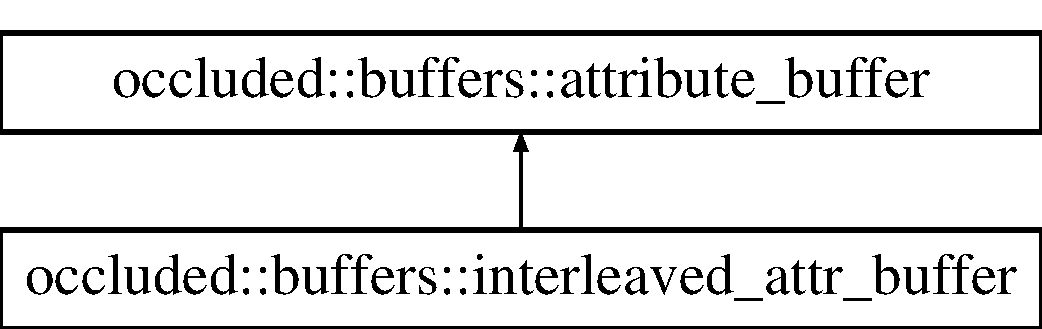
\includegraphics[height=2.000000cm]{classoccluded_1_1buffers_1_1interleaved__attr__buffer}
\end{center}
\end{figure}
\subsection*{Public Member Functions}
\begin{DoxyCompactItemize}
\item 
\hypertarget{classoccluded_1_1buffers_1_1interleaved__attr__buffer_af40be210a1b5468d1696e1cb1e9f663b}{{\bfseries interleaved\+\_\+attr\+\_\+buffer} (const \hyperlink{classoccluded_1_1buffers_1_1attributes_1_1attribute__map}{attributes\+::attribute\+\_\+map} \&map)}\label{classoccluded_1_1buffers_1_1interleaved__attr__buffer_af40be210a1b5468d1696e1cb1e9f663b}

\item 
void \hyperlink{classoccluded_1_1buffers_1_1interleaved__attr__buffer_a7347f20462c3bb9744602fc159e54e00}{insert\+\_\+values} (const std\+::vector$<$ char $>$ \&values)
\begin{DoxyCompactList}\small\item\em Inserts values into the attribute buffer. \end{DoxyCompactList}\end{DoxyCompactItemize}
\subsection*{Additional Inherited Members}


\subsection{Detailed Description}
An attribute buffer subclass with interleaved data. 

An attribute buffer that stores values such that they are interleaved. The first value of the first attribute will be stored then the first value of the second attribute will stored and so on. 

\subsection{Member Function Documentation}
\hypertarget{classoccluded_1_1buffers_1_1interleaved__attr__buffer_a7347f20462c3bb9744602fc159e54e00}{\index{occluded\+::buffers\+::interleaved\+\_\+attr\+\_\+buffer@{occluded\+::buffers\+::interleaved\+\_\+attr\+\_\+buffer}!insert\+\_\+values@{insert\+\_\+values}}
\index{insert\+\_\+values@{insert\+\_\+values}!occluded\+::buffers\+::interleaved\+\_\+attr\+\_\+buffer@{occluded\+::buffers\+::interleaved\+\_\+attr\+\_\+buffer}}
\subsubsection[{insert\+\_\+values}]{\setlength{\rightskip}{0pt plus 5cm}occluded\+::buffers\+::interleaved\+\_\+attr\+\_\+buffer\+::insert\+\_\+values (
\begin{DoxyParamCaption}
\item[{const std\+::vector$<$ char $>$ \&}]{values}
\end{DoxyParamCaption}
)\hspace{0.3cm}{\ttfamily [virtual]}}}\label{classoccluded_1_1buffers_1_1interleaved__attr__buffer_a7347f20462c3bb9744602fc159e54e00}


Inserts values into the attribute buffer. 


\begin{DoxyParams}{Parameters}
{\em values} & A reference to a vector of characters representing the values to be inserted.\\
\hline
\end{DoxyParams}
Inserts a value into the attribute buffer. Since the attribute values are interleaved and the vector passed as a parameter has interleaved values, the values can be placed as the end of the buffer. 

Implements \hyperlink{classoccluded_1_1buffers_1_1attribute__buffer_a323a2283330b0bcf4909e8d93bfc594a}{occluded\+::buffers\+::attribute\+\_\+buffer}.



The documentation for this class was generated from the following files\+:\begin{DoxyCompactItemize}
\item 
Occluded\+Library/buffers/interleaved\+\_\+attr\+\_\+buffer.\+h\item 
Occluded\+Library/buffers/interleaved\+\_\+attr\+\_\+buffer.\+cpp\end{DoxyCompactItemize}

\hypertarget{classoccluded_1_1meshes_1_1mesh}{\section{occluded\+:\+:meshes\+:\+:mesh Class Reference}
\label{classoccluded_1_1meshes_1_1mesh}\index{occluded\+::meshes\+::mesh@{occluded\+::meshes\+::mesh}}
}


An abstract class that provides an interface for all mesh classes.  




{\ttfamily \#include $<$mesh.\+h$>$}

Inheritance diagram for occluded\+:\+:meshes\+:\+:mesh\+:\begin{figure}[H]
\begin{center}
\leavevmode
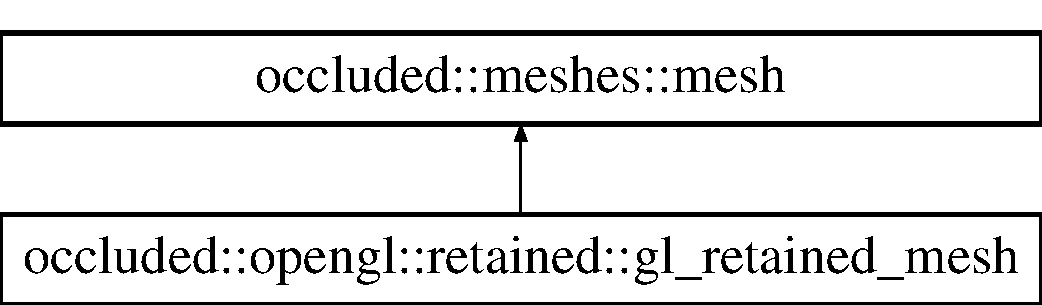
\includegraphics[height=2.000000cm]{classoccluded_1_1meshes_1_1mesh}
\end{center}
\end{figure}
\subsection*{Public Member Functions}
\begin{DoxyCompactItemize}
\item 
\hypertarget{classoccluded_1_1meshes_1_1mesh_a4249fa2a6e5482281aa7b4a48e8aa283}{\hyperlink{classoccluded_1_1meshes_1_1mesh_a4249fa2a6e5482281aa7b4a48e8aa283}{mesh} ()}\label{classoccluded_1_1meshes_1_1mesh_a4249fa2a6e5482281aa7b4a48e8aa283}

\begin{DoxyCompactList}\small\item\em Initializes the mesh. \end{DoxyCompactList}\item 
virtual void \hyperlink{classoccluded_1_1meshes_1_1mesh_ac9b5fa42ac4d6e2da862311058b664d6}{draw} () const =0
\begin{DoxyCompactList}\small\item\em Draws the mesh. \end{DoxyCompactList}\item 
virtual const std\+::vector\\*
$<$ unsigned int $>$ \hyperlink{classoccluded_1_1meshes_1_1mesh_ad015481328fc0ae9f72712f7f58ef1e3}{add\+\_\+vertices} (const std\+::vector$<$ char $>$ \&vertices)=0
\begin{DoxyCompactList}\small\item\em Adds vertices to the mesh. \end{DoxyCompactList}\item 
virtual const unsigned int \hyperlink{classoccluded_1_1meshes_1_1mesh_a4be1ad0c1b5144faa4f0e9a9c1d3023b}{add\+\_\+face} (const std\+::vector$<$ unsigned int $>$ \&face\+Indices)=0
\begin{DoxyCompactList}\small\item\em Adds a single face to the mesh. \end{DoxyCompactList}\item 
virtual const unsigned int \hyperlink{classoccluded_1_1meshes_1_1mesh_a70fbac683f8718017fde9236c7c0b156}{num\+\_\+verts\+\_\+for\+\_\+next\+\_\+face} (const unsigned int num\+Faces) const =0
\begin{DoxyCompactList}\small\item\em Gets the number of vertices needed for the next face. \end{DoxyCompactList}\end{DoxyCompactItemize}


\subsection{Detailed Description}
An abstract class that provides an interface for all mesh classes. 

An abstract class that provides an interface for all mesh classes. Since meshes are one of the basic objects that will be used in the occluded library, a common interface must be created for all meshes so that any graphics A\+P\+I can be used without changing the way in which the library is used by the end user. 

\subsection{Member Function Documentation}
\hypertarget{classoccluded_1_1meshes_1_1mesh_a4be1ad0c1b5144faa4f0e9a9c1d3023b}{\index{occluded\+::meshes\+::mesh@{occluded\+::meshes\+::mesh}!add\+\_\+face@{add\+\_\+face}}
\index{add\+\_\+face@{add\+\_\+face}!occluded\+::meshes\+::mesh@{occluded\+::meshes\+::mesh}}
\subsubsection[{add\+\_\+face}]{\setlength{\rightskip}{0pt plus 5cm}occluded\+::meshes\+::mesh\+::add\+\_\+face (
\begin{DoxyParamCaption}
\item[{const std\+::vector$<$ unsigned int $>$ \&}]{face\+Indices}
\end{DoxyParamCaption}
)\hspace{0.3cm}{\ttfamily [pure virtual]}}}\label{classoccluded_1_1meshes_1_1mesh_a4be1ad0c1b5144faa4f0e9a9c1d3023b}


Adds a single face to the mesh. 


\begin{DoxyParams}{Parameters}
{\em face\+Indices} & A reference to a vector of unsigned ints containing the indices of the vertices that make up the face to be added. \\
\hline
\end{DoxyParams}
\begin{DoxyReturn}{Returns}
A unsigned int representing the index of the face that was added.
\end{DoxyReturn}
Adds a face to the mesh that is made up of the vertices specified by the indices in the face\+Indices vector. An exception is thrown if the face\+Indices vector does not contain the correct number of vertices or if it contains a index that does not correspond to a vertex in the the mesh. 

Implemented in \hyperlink{classoccluded_1_1opengl_1_1retained_1_1gl__retained__mesh_ae9f8c756698b09458d61aba3a616f78b}{occluded\+::opengl\+::retained\+::gl\+\_\+retained\+\_\+mesh}.

\hypertarget{classoccluded_1_1meshes_1_1mesh_ad015481328fc0ae9f72712f7f58ef1e3}{\index{occluded\+::meshes\+::mesh@{occluded\+::meshes\+::mesh}!add\+\_\+vertices@{add\+\_\+vertices}}
\index{add\+\_\+vertices@{add\+\_\+vertices}!occluded\+::meshes\+::mesh@{occluded\+::meshes\+::mesh}}
\subsubsection[{add\+\_\+vertices}]{\setlength{\rightskip}{0pt plus 5cm}occluded\+::meshes\+::mesh\+::add\+\_\+vertices (
\begin{DoxyParamCaption}
\item[{const std\+::vector$<$ char $>$ \&}]{vertices}
\end{DoxyParamCaption}
)\hspace{0.3cm}{\ttfamily [pure virtual]}}}\label{classoccluded_1_1meshes_1_1mesh_ad015481328fc0ae9f72712f7f58ef1e3}


Adds vertices to the mesh. 


\begin{DoxyParams}{Parameters}
{\em vertices} & A reference to a vector of bytes. \\
\hline
\end{DoxyParams}
\begin{DoxyReturn}{Returns}
A vector of unsigned ints representing the indices of the vertices added.
\end{DoxyReturn}
Adds the vertices contained in the vector to the mesh. An exception will be thrown if the vertices vector is not formatted to be properly inserted into the data structure that is to contain the data. 

Implemented in \hyperlink{classoccluded_1_1opengl_1_1retained_1_1gl__retained__mesh_af1df11c76aefccc2bd9b67f839bfcbb8}{occluded\+::opengl\+::retained\+::gl\+\_\+retained\+\_\+mesh}.

\hypertarget{classoccluded_1_1meshes_1_1mesh_ac9b5fa42ac4d6e2da862311058b664d6}{\index{occluded\+::meshes\+::mesh@{occluded\+::meshes\+::mesh}!draw@{draw}}
\index{draw@{draw}!occluded\+::meshes\+::mesh@{occluded\+::meshes\+::mesh}}
\subsubsection[{draw}]{\setlength{\rightskip}{0pt plus 5cm}occluded\+::meshes\+::mesh\+::draw (
\begin{DoxyParamCaption}
{}
\end{DoxyParamCaption}
) const\hspace{0.3cm}{\ttfamily [pure virtual]}}}\label{classoccluded_1_1meshes_1_1mesh_ac9b5fa42ac4d6e2da862311058b664d6}


Draws the mesh. 

Draws the mesh to the context. 

Implemented in \hyperlink{classoccluded_1_1opengl_1_1retained_1_1gl__retained__mesh_aa2018120d3a1dcca990e85a24efe20fb}{occluded\+::opengl\+::retained\+::gl\+\_\+retained\+\_\+mesh}.

\hypertarget{classoccluded_1_1meshes_1_1mesh_a70fbac683f8718017fde9236c7c0b156}{\index{occluded\+::meshes\+::mesh@{occluded\+::meshes\+::mesh}!num\+\_\+verts\+\_\+for\+\_\+next\+\_\+face@{num\+\_\+verts\+\_\+for\+\_\+next\+\_\+face}}
\index{num\+\_\+verts\+\_\+for\+\_\+next\+\_\+face@{num\+\_\+verts\+\_\+for\+\_\+next\+\_\+face}!occluded\+::meshes\+::mesh@{occluded\+::meshes\+::mesh}}
\subsubsection[{num\+\_\+verts\+\_\+for\+\_\+next\+\_\+face}]{\setlength{\rightskip}{0pt plus 5cm}occluded\+::meshes\+::mesh\+::num\+\_\+verts\+\_\+for\+\_\+next\+\_\+face (
\begin{DoxyParamCaption}
\item[{const unsigned int}]{num\+Faces}
\end{DoxyParamCaption}
) const\hspace{0.3cm}{\ttfamily [pure virtual]}}}\label{classoccluded_1_1meshes_1_1mesh_a70fbac683f8718017fde9236c7c0b156}


Gets the number of vertices needed for the next face. 


\begin{DoxyParams}{Parameters}
{\em num\+Faces} & An unsigned int that specifies a face in the mesh. \\
\hline
\end{DoxyParams}
\begin{DoxyReturn}{Returns}
Returns an unsigned int representing the number of vertices needed to add a new face.
\end{DoxyReturn}
Gets the number of vertices needed for the next face to be added to the mesh after the face specified by num\+Faces parameter. This should be called before adding a face to the mesh so that the chance of an exception being thrown by the call is minimized. 

Implemented in \hyperlink{classoccluded_1_1opengl_1_1retained_1_1gl__retained__mesh_ab3efafd282bb6f844bd21ca911cfe9dd}{occluded\+::opengl\+::retained\+::gl\+\_\+retained\+\_\+mesh}.



The documentation for this class was generated from the following file\+:\begin{DoxyCompactItemize}
\item 
Occluded\+Library/meshes/mesh.\+h\end{DoxyCompactItemize}

\hypertarget{classoccluded_1_1buffers_1_1segregated__attr__buffer}{\section{occluded\+:\+:buffers\+:\+:segregated\+\_\+attr\+\_\+buffer Class Reference}
\label{classoccluded_1_1buffers_1_1segregated__attr__buffer}\index{occluded\+::buffers\+::segregated\+\_\+attr\+\_\+buffer@{occluded\+::buffers\+::segregated\+\_\+attr\+\_\+buffer}}
}


An attribute buffer subclass with segregated data.  




{\ttfamily \#include $<$segregated\+\_\+attr\+\_\+buffer.\+h$>$}

Inheritance diagram for occluded\+:\+:buffers\+:\+:segregated\+\_\+attr\+\_\+buffer\+:\begin{figure}[H]
\begin{center}
\leavevmode
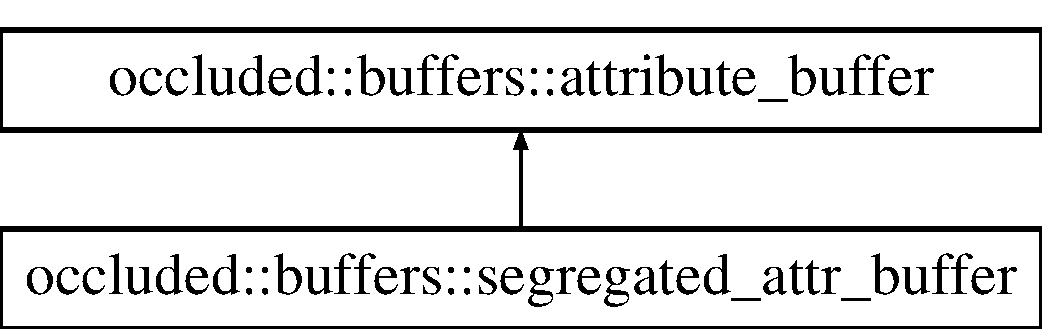
\includegraphics[height=2.000000cm]{classoccluded_1_1buffers_1_1segregated__attr__buffer}
\end{center}
\end{figure}
\subsection*{Public Member Functions}
\begin{DoxyCompactItemize}
\item 
\hyperlink{classoccluded_1_1buffers_1_1segregated__attr__buffer_ab822a9e4ccf2be069418224fc2663622}{segregated\+\_\+attr\+\_\+buffer} (const \hyperlink{classoccluded_1_1buffers_1_1attributes_1_1attribute__map}{attributes\+::attribute\+\_\+map} \&map)
\begin{DoxyCompactList}\small\item\em Initializes the attribute buffer. \end{DoxyCompactList}\item 
void \hyperlink{classoccluded_1_1buffers_1_1segregated__attr__buffer_a437ef88504021dc75d45dff010986128}{insert\+\_\+values} (const std\+::vector$<$ char $>$ \&values)
\begin{DoxyCompactList}\small\item\em Inserts values into the attribute buffer. \end{DoxyCompactList}\end{DoxyCompactItemize}
\subsection*{Additional Inherited Members}


\subsection{Detailed Description}
An attribute buffer subclass with segregated data. 

An attribute buffer that stores values in segregated sections. The first value of the first attribute will be stored, then the second value of the first attribute is stored and so on. 

\subsection{Constructor \& Destructor Documentation}
\hypertarget{classoccluded_1_1buffers_1_1segregated__attr__buffer_ab822a9e4ccf2be069418224fc2663622}{\index{occluded\+::buffers\+::segregated\+\_\+attr\+\_\+buffer@{occluded\+::buffers\+::segregated\+\_\+attr\+\_\+buffer}!segregated\+\_\+attr\+\_\+buffer@{segregated\+\_\+attr\+\_\+buffer}}
\index{segregated\+\_\+attr\+\_\+buffer@{segregated\+\_\+attr\+\_\+buffer}!occluded\+::buffers\+::segregated\+\_\+attr\+\_\+buffer@{occluded\+::buffers\+::segregated\+\_\+attr\+\_\+buffer}}
\subsubsection[{segregated\+\_\+attr\+\_\+buffer}]{\setlength{\rightskip}{0pt plus 5cm}occluded\+::buffers\+::segregated\+\_\+attr\+\_\+buffer\+::segregated\+\_\+attr\+\_\+buffer (
\begin{DoxyParamCaption}
\item[{const {\bf attributes\+::attribute\+\_\+map} \&}]{map}
\end{DoxyParamCaption}
)}}\label{classoccluded_1_1buffers_1_1segregated__attr__buffer_ab822a9e4ccf2be069418224fc2663622}


Initializes the attribute buffer. 


\begin{DoxyParams}{Parameters}
{\em map} & A reference to an attribute map.\\
\hline
\end{DoxyParams}
Initializes the attribute buffer. Throws an exception if the map is not a segregated map. 

\subsection{Member Function Documentation}
\hypertarget{classoccluded_1_1buffers_1_1segregated__attr__buffer_a437ef88504021dc75d45dff010986128}{\index{occluded\+::buffers\+::segregated\+\_\+attr\+\_\+buffer@{occluded\+::buffers\+::segregated\+\_\+attr\+\_\+buffer}!insert\+\_\+values@{insert\+\_\+values}}
\index{insert\+\_\+values@{insert\+\_\+values}!occluded\+::buffers\+::segregated\+\_\+attr\+\_\+buffer@{occluded\+::buffers\+::segregated\+\_\+attr\+\_\+buffer}}
\subsubsection[{insert\+\_\+values}]{\setlength{\rightskip}{0pt plus 5cm}occluded\+::buffers\+::segregated\+\_\+attr\+\_\+buffer\+::insert\+\_\+values (
\begin{DoxyParamCaption}
\item[{const std\+::vector$<$ char $>$ \&}]{values}
\end{DoxyParamCaption}
)\hspace{0.3cm}{\ttfamily [virtual]}}}\label{classoccluded_1_1buffers_1_1segregated__attr__buffer_a437ef88504021dc75d45dff010986128}


Inserts values into the attribute buffer. 


\begin{DoxyParams}{Parameters}
{\em values} & A reference to a vector of characters representing the values to be inserted.\\
\hline
\end{DoxyParams}
Inserts a value into the attribute buffer. The values in the vector parameter will be split up and each value will be placed in the correct section of the buffer. 

Implements \hyperlink{classoccluded_1_1buffers_1_1attribute__buffer_a323a2283330b0bcf4909e8d93bfc594a}{occluded\+::buffers\+::attribute\+\_\+buffer}.



The documentation for this class was generated from the following files\+:\begin{DoxyCompactItemize}
\item 
Occluded\+Library/buffers/segregated\+\_\+attr\+\_\+buffer.\+h\item 
Occluded\+Library/buffers/segregated\+\_\+attr\+\_\+buffer.\+cpp\end{DoxyCompactItemize}

\hypertarget{classoccluded_1_1opengl_1_1retained_1_1shaders_1_1shader}{\section{occluded\+:\+:opengl\+:\+:retained\+:\+:shaders\+:\+:shader Class Reference}
\label{classoccluded_1_1opengl_1_1retained_1_1shaders_1_1shader}\index{occluded\+::opengl\+::retained\+::shaders\+::shader@{occluded\+::opengl\+::retained\+::shaders\+::shader}}
}


A wrapper class for an Open\+G\+L shader.  




{\ttfamily \#include $<$shader.\+h$>$}

\subsection*{Public Member Functions}
\begin{DoxyCompactItemize}
\item 
\hyperlink{classoccluded_1_1opengl_1_1retained_1_1shaders_1_1shader_ac40b834734bf03a1c060f771b1741823}{shader} (const std\+::string \&shader\+Src, const shader\+\_\+type\+\_\+t type)
\begin{DoxyCompactList}\small\item\em Initializes and compiles the shader. \end{DoxyCompactList}\item 
const G\+Luint \hyperlink{classoccluded_1_1opengl_1_1retained_1_1shaders_1_1shader_a1694ca35f6ad85cf95a3f6b3c7b783e3}{get\+\_\+id} () const 
\begin{DoxyCompactList}\small\item\em Gets the id of the shader. \end{DoxyCompactList}\item 
const bool \hyperlink{classoccluded_1_1opengl_1_1retained_1_1shaders_1_1shader_af1fe3fdd511da901ffa7665dad8a1d12}{is\+\_\+compiled} () const 
\begin{DoxyCompactList}\small\item\em Returns true if the shader is compiled, and false otherwise. \end{DoxyCompactList}\item 
const shader\+\_\+type\+\_\+t \hyperlink{classoccluded_1_1opengl_1_1retained_1_1shaders_1_1shader_af9befeaa32ea72f80d1c3825f4cd2f48}{get\+\_\+type} () const 
\begin{DoxyCompactList}\small\item\em Gets the type of the shader. \end{DoxyCompactList}\item 
const std\+::string \& \hyperlink{classoccluded_1_1opengl_1_1retained_1_1shaders_1_1shader_add6cda8459eb2a802e8eb22f70bbd1db}{get\+\_\+compile\+\_\+log} () const 
\begin{DoxyCompactList}\small\item\em Gets the compile log if a compilation error occurs. \end{DoxyCompactList}\end{DoxyCompactItemize}


\subsection{Detailed Description}
A wrapper class for an Open\+G\+L shader. 

A wrapper class for an Open\+G\+L G\+L\+S\+L shader. This is class holds information necessary for creating a G\+L\+S\+L shader as well as making it easy for accessing information about a compiled shader without having to query Open\+G\+L. It also allows for determining if a shader has not compiled properly and for accessing the error log to examine the compilation errors. 

\subsection{Constructor \& Destructor Documentation}
\hypertarget{classoccluded_1_1opengl_1_1retained_1_1shaders_1_1shader_ac40b834734bf03a1c060f771b1741823}{\index{occluded\+::opengl\+::retained\+::shaders\+::shader@{occluded\+::opengl\+::retained\+::shaders\+::shader}!shader@{shader}}
\index{shader@{shader}!occluded\+::opengl\+::retained\+::shaders\+::shader@{occluded\+::opengl\+::retained\+::shaders\+::shader}}
\subsubsection[{shader}]{\setlength{\rightskip}{0pt plus 5cm}occluded\+::opengl\+::retained\+::shaders\+::shader\+::shader (
\begin{DoxyParamCaption}
\item[{const std\+::string \&}]{shader\+Src, }
\item[{const shader\+\_\+type\+\_\+t}]{type}
\end{DoxyParamCaption}
)}}\label{classoccluded_1_1opengl_1_1retained_1_1shaders_1_1shader_ac40b834734bf03a1c060f771b1741823}


Initializes and compiles the shader. 


\begin{DoxyParams}{Parameters}
{\em shader\+Src} & A reference to a string containing the source code of the G\+L\+S\+L shader. \\
\hline
{\em type} & The type of this G\+L\+S\+L shader.\\
\hline
\end{DoxyParams}
Initializes and compiles the shader program specified by the shader source and the shader type provided. If the shader has a problem compiling, the compile log will be stored and an exception will be thrown. 

\subsection{Member Function Documentation}
\hypertarget{classoccluded_1_1opengl_1_1retained_1_1shaders_1_1shader_add6cda8459eb2a802e8eb22f70bbd1db}{\index{occluded\+::opengl\+::retained\+::shaders\+::shader@{occluded\+::opengl\+::retained\+::shaders\+::shader}!get\+\_\+compile\+\_\+log@{get\+\_\+compile\+\_\+log}}
\index{get\+\_\+compile\+\_\+log@{get\+\_\+compile\+\_\+log}!occluded\+::opengl\+::retained\+::shaders\+::shader@{occluded\+::opengl\+::retained\+::shaders\+::shader}}
\subsubsection[{get\+\_\+compile\+\_\+log}]{\setlength{\rightskip}{0pt plus 5cm}occluded\+::opengl\+::retained\+::shaders\+::shader\+::get\+\_\+compile\+\_\+log (
\begin{DoxyParamCaption}
{}
\end{DoxyParamCaption}
) const}}\label{classoccluded_1_1opengl_1_1retained_1_1shaders_1_1shader_add6cda8459eb2a802e8eb22f70bbd1db}


Gets the compile log if a compilation error occurs. 

\begin{DoxyReturn}{Returns}
Returns a reference to the string containing the shader's compile log.
\end{DoxyReturn}
Gets the the compile log of the G\+L\+S\+L shader if there is a problem during compilation. If there was no problem during compilation, an exception will be thrown. \hypertarget{classoccluded_1_1opengl_1_1retained_1_1shaders_1_1shader_a1694ca35f6ad85cf95a3f6b3c7b783e3}{\index{occluded\+::opengl\+::retained\+::shaders\+::shader@{occluded\+::opengl\+::retained\+::shaders\+::shader}!get\+\_\+id@{get\+\_\+id}}
\index{get\+\_\+id@{get\+\_\+id}!occluded\+::opengl\+::retained\+::shaders\+::shader@{occluded\+::opengl\+::retained\+::shaders\+::shader}}
\subsubsection[{get\+\_\+id}]{\setlength{\rightskip}{0pt plus 5cm}occluded\+::opengl\+::retained\+::shaders\+::shader\+::get\+\_\+id (
\begin{DoxyParamCaption}
{}
\end{DoxyParamCaption}
) const}}\label{classoccluded_1_1opengl_1_1retained_1_1shaders_1_1shader_a1694ca35f6ad85cf95a3f6b3c7b783e3}


Gets the id of the shader. 

\begin{DoxyReturn}{Returns}
Returns the id of the G\+L\+S\+L shader.
\end{DoxyReturn}
Gets the id of the G\+L\+S\+L shader and throws an exception if an error occured during shader compilation. \hypertarget{classoccluded_1_1opengl_1_1retained_1_1shaders_1_1shader_af9befeaa32ea72f80d1c3825f4cd2f48}{\index{occluded\+::opengl\+::retained\+::shaders\+::shader@{occluded\+::opengl\+::retained\+::shaders\+::shader}!get\+\_\+type@{get\+\_\+type}}
\index{get\+\_\+type@{get\+\_\+type}!occluded\+::opengl\+::retained\+::shaders\+::shader@{occluded\+::opengl\+::retained\+::shaders\+::shader}}
\subsubsection[{get\+\_\+type}]{\setlength{\rightskip}{0pt plus 5cm}occluded\+::opengl\+::retained\+::shaders\+::shader\+::get\+\_\+type (
\begin{DoxyParamCaption}
{}
\end{DoxyParamCaption}
) const}}\label{classoccluded_1_1opengl_1_1retained_1_1shaders_1_1shader_af9befeaa32ea72f80d1c3825f4cd2f48}


Gets the type of the shader. 

\begin{DoxyReturn}{Returns}
Returns a shader\+\_\+type\+\_\+t representing the shader's type.
\end{DoxyReturn}
Gets the shader\+\_\+type\+\_\+t of the shader. Used to prevent problems with incorrect types of shaders being used in the same \hyperlink{classoccluded_1_1opengl_1_1retained_1_1shaders_1_1shader__program}{shader\+\_\+program}. \hypertarget{classoccluded_1_1opengl_1_1retained_1_1shaders_1_1shader_af1fe3fdd511da901ffa7665dad8a1d12}{\index{occluded\+::opengl\+::retained\+::shaders\+::shader@{occluded\+::opengl\+::retained\+::shaders\+::shader}!is\+\_\+compiled@{is\+\_\+compiled}}
\index{is\+\_\+compiled@{is\+\_\+compiled}!occluded\+::opengl\+::retained\+::shaders\+::shader@{occluded\+::opengl\+::retained\+::shaders\+::shader}}
\subsubsection[{is\+\_\+compiled}]{\setlength{\rightskip}{0pt plus 5cm}occluded\+::opengl\+::retained\+::shaders\+::shader\+::is\+\_\+compiled (
\begin{DoxyParamCaption}
{}
\end{DoxyParamCaption}
) const}}\label{classoccluded_1_1opengl_1_1retained_1_1shaders_1_1shader_af1fe3fdd511da901ffa7665dad8a1d12}


Returns true if the shader is compiled, and false otherwise. 

\begin{DoxyReturn}{Returns}
Returns whether or not the shader is compiled.
\end{DoxyReturn}
Returns true if the G\+L\+S\+L is compiled and false if an error occured during compilation. This is used to quickly determine if a shader can be used in a G\+L\+S\+L shader program. 

The documentation for this class was generated from the following files\+:\begin{DoxyCompactItemize}
\item 
Occluded\+Library/opengl/retained/shaders/shader.\+h\item 
Occluded\+Library/opengl/retained/shaders/shader.\+cpp\end{DoxyCompactItemize}

\hypertarget{classoccluded_1_1opengl_1_1retained_1_1shaders_1_1shader__attribute__map}{\section{occluded\+:\+:opengl\+:\+:retained\+:\+:shaders\+:\+:shader\+\_\+attribute\+\_\+map Class Reference}
\label{classoccluded_1_1opengl_1_1retained_1_1shaders_1_1shader__attribute__map}\index{occluded\+::opengl\+::retained\+::shaders\+::shader\+\_\+attribute\+\_\+map@{occluded\+::opengl\+::retained\+::shaders\+::shader\+\_\+attribute\+\_\+map}}
}


Handles the mapping of attributes in an attribute map to those in a shader program.  




{\ttfamily \#include $<$shader\+\_\+attribute\+\_\+map.\+h$>$}

\subsection*{Public Member Functions}
\begin{DoxyCompactItemize}
\item 
\hyperlink{classoccluded_1_1opengl_1_1retained_1_1shaders_1_1shader__attribute__map_a317ce382cc4aabad2ba440a2bc0ab745}{shader\+\_\+attribute\+\_\+map} (const \hyperlink{classoccluded_1_1buffers_1_1attributes_1_1attribute__map}{buffers\+::attributes\+::attribute\+\_\+map} \&map, const \hyperlink{classoccluded_1_1opengl_1_1retained_1_1shaders_1_1shader__program}{shader\+\_\+program} \&shader\+Prog)
\begin{DoxyCompactList}\small\item\em Initializes the shader attribute map. \end{DoxyCompactList}\item 
void \hyperlink{classoccluded_1_1opengl_1_1retained_1_1shaders_1_1shader__attribute__map_a913681eba3098eae202cc8aee51fdb71}{set\+\_\+attrib\+\_\+pointers} (const \hyperlink{classoccluded_1_1buffers_1_1attribute__buffer}{buffers\+::attribute\+\_\+buffer} \&buffer) const 
\begin{DoxyCompactList}\small\item\em Setups of all the vertex attrib pointers in preparation for a draw call. \end{DoxyCompactList}\end{DoxyCompactItemize}


\subsection{Detailed Description}
Handles the mapping of attributes in an attribute map to those in a shader program. 

This handles the mapping of attribute in an attribute map to those in a shader program. Its purpose is to reduce all the calls to gl\+Vertex\+Attrib\+Pointer to a single a function call as well as to prevent calls to gl\+Vertex\+Attrib\+Pointer that would cause Open\+G\+L to enter an error state. 

\subsection{Constructor \& Destructor Documentation}
\hypertarget{classoccluded_1_1opengl_1_1retained_1_1shaders_1_1shader__attribute__map_a317ce382cc4aabad2ba440a2bc0ab745}{\index{occluded\+::opengl\+::retained\+::shaders\+::shader\+\_\+attribute\+\_\+map@{occluded\+::opengl\+::retained\+::shaders\+::shader\+\_\+attribute\+\_\+map}!shader\+\_\+attribute\+\_\+map@{shader\+\_\+attribute\+\_\+map}}
\index{shader\+\_\+attribute\+\_\+map@{shader\+\_\+attribute\+\_\+map}!occluded\+::opengl\+::retained\+::shaders\+::shader\+\_\+attribute\+\_\+map@{occluded\+::opengl\+::retained\+::shaders\+::shader\+\_\+attribute\+\_\+map}}
\subsubsection[{shader\+\_\+attribute\+\_\+map}]{\setlength{\rightskip}{0pt plus 5cm}occluded\+::opengl\+::retained\+::shaders\+::shader\+\_\+attribute\+\_\+map\+::shader\+\_\+attribute\+\_\+map (
\begin{DoxyParamCaption}
\item[{const {\bf buffers\+::attributes\+::attribute\+\_\+map} \&}]{map, }
\item[{const {\bf shader\+\_\+program} \&}]{shader\+Prog}
\end{DoxyParamCaption}
)}}\label{classoccluded_1_1opengl_1_1retained_1_1shaders_1_1shader__attribute__map_a317ce382cc4aabad2ba440a2bc0ab745}


Initializes the shader attribute map. 


\begin{DoxyParams}{Parameters}
{\em map} & A reference to an attribute map. \\
\hline
{\em shader\+Prog} & A reference to a shader program.\\
\hline
\end{DoxyParams}
Initializes the shader attribute map, by determining which attributes are active attributes in shader program and storing their a mapping from the name of the attribute to the id of the Open\+G\+L attribute. A -\/1 will stored if the attribute does not exist in the shader program. \begin{DoxyWarning}{Warning}
\{ The convention is for an attribute named \char`\"{}position\char`\"{} in the attribute map will search for \char`\"{}v\+Position\char`\"{} attribute in the shader program. This v is to indicate that the attribute is part of the vertex shader and meant to help in quickly locating it. \} 
\end{DoxyWarning}


\subsection{Member Function Documentation}
\hypertarget{classoccluded_1_1opengl_1_1retained_1_1shaders_1_1shader__attribute__map_a913681eba3098eae202cc8aee51fdb71}{\index{occluded\+::opengl\+::retained\+::shaders\+::shader\+\_\+attribute\+\_\+map@{occluded\+::opengl\+::retained\+::shaders\+::shader\+\_\+attribute\+\_\+map}!set\+\_\+attrib\+\_\+pointers@{set\+\_\+attrib\+\_\+pointers}}
\index{set\+\_\+attrib\+\_\+pointers@{set\+\_\+attrib\+\_\+pointers}!occluded\+::opengl\+::retained\+::shaders\+::shader\+\_\+attribute\+\_\+map@{occluded\+::opengl\+::retained\+::shaders\+::shader\+\_\+attribute\+\_\+map}}
\subsubsection[{set\+\_\+attrib\+\_\+pointers}]{\setlength{\rightskip}{0pt plus 5cm}occluded\+::opengl\+::retained\+::shaders\+::shader\+\_\+attribute\+\_\+map\+::set\+\_\+attrib\+\_\+pointers (
\begin{DoxyParamCaption}
\item[{const {\bf buffers\+::attribute\+\_\+buffer} \&}]{buffer}
\end{DoxyParamCaption}
) const}}\label{classoccluded_1_1opengl_1_1retained_1_1shaders_1_1shader__attribute__map_a913681eba3098eae202cc8aee51fdb71}


Setups of all the vertex attrib pointers in preparation for a draw call. 


\begin{DoxyParams}{Parameters}
{\em buffer} & The attribute buffer the attrib pointers will be set for.\\
\hline
\end{DoxyParams}
Makes all the necessary calls to gl\+Vertex\+Attrib\+Pointer that are needed in order to make a gl\+Draw call. Used the necessary preparation for an Open\+G\+L buffer object, thats data is organized according to the attribute\+\_\+map, to be used by a gl\+Draw call. 

The documentation for this class was generated from the following files\+:\begin{DoxyCompactItemize}
\item 
Occluded\+Library/opengl/retained/shaders/shader\+\_\+attribute\+\_\+map.\+h\item 
Occluded\+Library/opengl/retained/shaders/shader\+\_\+attribute\+\_\+map.\+cpp\end{DoxyCompactItemize}

\hypertarget{classoccluded_1_1opengl_1_1retained_1_1shaders_1_1shader__program}{\section{occluded\+:\+:opengl\+:\+:retained\+:\+:shaders\+:\+:shader\+\_\+program Class Reference}
\label{classoccluded_1_1opengl_1_1retained_1_1shaders_1_1shader__program}\index{occluded\+::opengl\+::retained\+::shaders\+::shader\+\_\+program@{occluded\+::opengl\+::retained\+::shaders\+::shader\+\_\+program}}
}


A wrapper class for an Open\+G\+L G\+L\+S\+L shader program.  




{\ttfamily \#include $<$shader\+\_\+program.\+h$>$}

\subsection*{Public Member Functions}
\begin{DoxyCompactItemize}
\item 
\hyperlink{classoccluded_1_1opengl_1_1retained_1_1shaders_1_1shader__program_a940103083cf5b991c8de690748311dc3}{shader\+\_\+program} ()
\begin{DoxyCompactList}\small\item\em Creates an empty shader program that cannot be used for rendering. \end{DoxyCompactList}\item 
\hyperlink{classoccluded_1_1opengl_1_1retained_1_1shaders_1_1shader__program_ab866c58d6541142d873e0ec532fd194a}{shader\+\_\+program} (const std\+::vector$<$ \hyperlink{classoccluded_1_1opengl_1_1retained_1_1shaders_1_1shader}{shader} $>$ \&shaders)
\begin{DoxyCompactList}\small\item\em Creates and initializes a Open\+G\+L G\+L\+S\+L shader program. \end{DoxyCompactList}\item 
void \hyperlink{classoccluded_1_1opengl_1_1retained_1_1shaders_1_1shader__program_a92731484e3b37d25b3dc66a3a1871d2e}{use\+\_\+program} () const 
\begin{DoxyCompactList}\small\item\em Tells Open\+G\+L to use the shader program. \end{DoxyCompactList}\item 
const G\+Luint \hyperlink{classoccluded_1_1opengl_1_1retained_1_1shaders_1_1shader__program_a5824dc0a31ac6e1100cfa0677e309020}{get\+\_\+id} () const 
\begin{DoxyCompactList}\small\item\em Gets the id of the shader program. \end{DoxyCompactList}\item 
\hypertarget{classoccluded_1_1opengl_1_1retained_1_1shaders_1_1shader__program_af713d427fa3e7a05ccee96cee435a100}{const bool {\bfseries is\+\_\+linked} () const }\label{classoccluded_1_1opengl_1_1retained_1_1shaders_1_1shader__program_af713d427fa3e7a05ccee96cee435a100}

\item 
\hypertarget{classoccluded_1_1opengl_1_1retained_1_1shaders_1_1shader__program_af2eb6bffe5e771bf47013086ace9d16f}{const std\+::string \& {\bfseries get\+\_\+error\+\_\+log} () const }\label{classoccluded_1_1opengl_1_1retained_1_1shaders_1_1shader__program_af2eb6bffe5e771bf47013086ace9d16f}

\end{DoxyCompactItemize}


\subsection{Detailed Description}
A wrapper class for an Open\+G\+L G\+L\+S\+L shader program. 

A wrapper class for an Open\+G\+L G\+L\+S\+L shader program. Used to create, attach shaders to, link, and use a shader program as well as to store and quickly access information about a shader program with out having to query Open\+G\+L directly. It also makes it easy to determine if a shader program is being used incorrectly by throwing exceptions when a function is called while the shader program is in the incorrect state or if invalid arguments are passed to it. 

\subsection{Constructor \& Destructor Documentation}
\hypertarget{classoccluded_1_1opengl_1_1retained_1_1shaders_1_1shader__program_a940103083cf5b991c8de690748311dc3}{\index{occluded\+::opengl\+::retained\+::shaders\+::shader\+\_\+program@{occluded\+::opengl\+::retained\+::shaders\+::shader\+\_\+program}!shader\+\_\+program@{shader\+\_\+program}}
\index{shader\+\_\+program@{shader\+\_\+program}!occluded\+::opengl\+::retained\+::shaders\+::shader\+\_\+program@{occluded\+::opengl\+::retained\+::shaders\+::shader\+\_\+program}}
\subsubsection[{shader\+\_\+program}]{\setlength{\rightskip}{0pt plus 5cm}occluded\+::opengl\+::retained\+::shaders\+::shader\+\_\+program\+::shader\+\_\+program (
\begin{DoxyParamCaption}
{}
\end{DoxyParamCaption}
)}}\label{classoccluded_1_1opengl_1_1retained_1_1shaders_1_1shader__program_a940103083cf5b991c8de690748311dc3}


Creates an empty shader program that cannot be used for rendering. 

Create an empty shader program that cannot be used for rendering. This is used to make it easier for the programmer to use and not violate the programming standards of his/her project. \hypertarget{classoccluded_1_1opengl_1_1retained_1_1shaders_1_1shader__program_ab866c58d6541142d873e0ec532fd194a}{\index{occluded\+::opengl\+::retained\+::shaders\+::shader\+\_\+program@{occluded\+::opengl\+::retained\+::shaders\+::shader\+\_\+program}!shader\+\_\+program@{shader\+\_\+program}}
\index{shader\+\_\+program@{shader\+\_\+program}!occluded\+::opengl\+::retained\+::shaders\+::shader\+\_\+program@{occluded\+::opengl\+::retained\+::shaders\+::shader\+\_\+program}}
\subsubsection[{shader\+\_\+program}]{\setlength{\rightskip}{0pt plus 5cm}occluded\+::opengl\+::retained\+::shaders\+::shader\+\_\+program\+::shader\+\_\+program (
\begin{DoxyParamCaption}
\item[{const std\+::vector$<$ {\bf shader} $>$ \&}]{shaders}
\end{DoxyParamCaption}
)}}\label{classoccluded_1_1opengl_1_1retained_1_1shaders_1_1shader__program_ab866c58d6541142d873e0ec532fd194a}


Creates and initializes a Open\+G\+L G\+L\+S\+L shader program. 


\begin{DoxyParams}{Parameters}
{\em shaders} & A vector of shaders that will be attached to the shader program.\\
\hline
\end{DoxyParams}
Creates a shader program, attaches the shaders in the shaders vector, and links the shader program. If everything works correctly the shader program can be used for rendering. If a problem occurs the an exception will be raised by this constructor. 

\subsection{Member Function Documentation}
\hypertarget{classoccluded_1_1opengl_1_1retained_1_1shaders_1_1shader__program_a5824dc0a31ac6e1100cfa0677e309020}{\index{occluded\+::opengl\+::retained\+::shaders\+::shader\+\_\+program@{occluded\+::opengl\+::retained\+::shaders\+::shader\+\_\+program}!get\+\_\+id@{get\+\_\+id}}
\index{get\+\_\+id@{get\+\_\+id}!occluded\+::opengl\+::retained\+::shaders\+::shader\+\_\+program@{occluded\+::opengl\+::retained\+::shaders\+::shader\+\_\+program}}
\subsubsection[{get\+\_\+id}]{\setlength{\rightskip}{0pt plus 5cm}occluded\+::opengl\+::retained\+::shaders\+::shader\+\_\+program\+::get\+\_\+id (
\begin{DoxyParamCaption}
{}
\end{DoxyParamCaption}
) const}}\label{classoccluded_1_1opengl_1_1retained_1_1shaders_1_1shader__program_a5824dc0a31ac6e1100cfa0677e309020}


Gets the id of the shader program. 

\begin{DoxyReturn}{Returns}
Returns the id of the Open\+G\+L G\+L\+S\+L shader program.
\end{DoxyReturn}
Returns the id of the Open\+G\+L G\+L\+S\+L shader program. This function will throw an exception if the shader program was not properly linked. This can be but should not be used to make a call to gl\+Use\+Program. Should be used for getting or binding the location of attributes and uniforms. \begin{DoxyWarning}{Warning}
Do not use for making a call to gl\+Delete\+Program because it will cause an error when the deconstructor tries to delete the program. 
\end{DoxyWarning}
\hypertarget{classoccluded_1_1opengl_1_1retained_1_1shaders_1_1shader__program_a92731484e3b37d25b3dc66a3a1871d2e}{\index{occluded\+::opengl\+::retained\+::shaders\+::shader\+\_\+program@{occluded\+::opengl\+::retained\+::shaders\+::shader\+\_\+program}!use\+\_\+program@{use\+\_\+program}}
\index{use\+\_\+program@{use\+\_\+program}!occluded\+::opengl\+::retained\+::shaders\+::shader\+\_\+program@{occluded\+::opengl\+::retained\+::shaders\+::shader\+\_\+program}}
\subsubsection[{use\+\_\+program}]{\setlength{\rightskip}{0pt plus 5cm}occluded\+::opengl\+::retained\+::shaders\+::shader\+\_\+program\+::use\+\_\+program (
\begin{DoxyParamCaption}
{}
\end{DoxyParamCaption}
) const}}\label{classoccluded_1_1opengl_1_1retained_1_1shaders_1_1shader__program_a92731484e3b37d25b3dc66a3a1871d2e}


Tells Open\+G\+L to use the shader program. 

Tells Open\+G\+L to use this G\+L\+S\+L shader program for rendering. This function will throw an exception if the shader program was not linked properly. Used to quickly tell the user that there is a problem with the shader program with out causing Open\+G\+L to enter an error state. 

The documentation for this class was generated from the following files\+:\begin{DoxyCompactItemize}
\item 
Occluded\+Library/opengl/retained/shaders/shader\+\_\+program.\+h\item 
Occluded\+Library/opengl/retained/shaders/shader\+\_\+program.\+cpp\end{DoxyCompactItemize}

\hypertarget{classoccluded_1_1opengl_1_1retained_1_1shaders_1_1shader__uniform__store}{\section{occluded\+:\+:opengl\+:\+:retained\+:\+:shaders\+:\+:shader\+\_\+uniform\+\_\+store Class Reference}
\label{classoccluded_1_1opengl_1_1retained_1_1shaders_1_1shader__uniform__store}\index{occluded\+::opengl\+::retained\+::shaders\+::shader\+\_\+uniform\+\_\+store@{occluded\+::opengl\+::retained\+::shaders\+::shader\+\_\+uniform\+\_\+store}}
}


Stores uniform values for a particular shader program.  




{\ttfamily \#include $<$shader\+\_\+uniform\+\_\+store.\+h$>$}

\subsection*{Public Member Functions}
\begin{DoxyCompactItemize}
\item 
\hyperlink{classoccluded_1_1opengl_1_1retained_1_1shaders_1_1shader__uniform__store_a862db8afb99f17ec1b14c3e9a882618e}{shader\+\_\+uniform\+\_\+store} (const \hyperlink{classoccluded_1_1opengl_1_1retained_1_1shaders_1_1shader__program}{shader\+\_\+program} \&shader\+Prog)
\begin{DoxyCompactList}\small\item\em Initializes an empty uniform store. \end{DoxyCompactList}\item 
\hyperlink{classoccluded_1_1opengl_1_1retained_1_1shaders_1_1shader__uniform__store_a7503a430211c435021dbbe9628cb4e40}{shader\+\_\+uniform\+\_\+store} (const \hyperlink{classoccluded_1_1opengl_1_1retained_1_1shaders_1_1shader__program}{shader\+\_\+program} \&shader\+Prog, const std\+::vector$<$ std\+::pair$<$ const std\+::string, const uniform\+\_\+value $>$ $>$ \&values)
\begin{DoxyCompactList}\small\item\em Initializes an uniform store and populates it. \end{DoxyCompactList}\item 
void \hyperlink{classoccluded_1_1opengl_1_1retained_1_1shaders_1_1shader__uniform__store_a3fb24f0d04b2f34c2013f9c272ba662b}{add\+\_\+uniform} (const std\+::string \&name, const uniform\+\_\+value \&value)
\begin{DoxyCompactList}\small\item\em Adds a new uniform value to the uniform store. \end{DoxyCompactList}\item 
void \hyperlink{classoccluded_1_1opengl_1_1retained_1_1shaders_1_1shader__uniform__store_adc43de912769b10941eb93b407d8662d}{set\+\_\+uniform\+\_\+value} (const std\+::string \&name, const uniform\+\_\+value \&value)
\begin{DoxyCompactList}\small\item\em Sets the value of a uniform. \end{DoxyCompactList}\item 
void \hyperlink{classoccluded_1_1opengl_1_1retained_1_1shaders_1_1shader__uniform__store_a3b451f197b65ba65077a8d2d368bae41}{pass\+\_\+to\+\_\+shader} () const 
\begin{DoxyCompactList}\small\item\em Passes the uniform values to the shader program. \end{DoxyCompactList}\item 
{\footnotesize template$<$typename T $>$ }\\const T \hyperlink{classoccluded_1_1opengl_1_1retained_1_1shaders_1_1shader__uniform__store_a69ee4a0dd33e31fcf4ea0e82acf0f2db}{get\+\_\+value} (const std\+::string \&name) const 
\begin{DoxyCompactList}\small\item\em Gets the value of a uniform. \end{DoxyCompactList}\end{DoxyCompactItemize}


\subsection{Detailed Description}
Stores uniform values for a particular shader program. 

Stores the uniform values for a particular shader program by maintaining a mapping from uniforms' names to their values. This class provides a way of storing all the uniform values of a \hyperlink{classoccluded_1_1opengl_1_1retained_1_1shaders_1_1shader__program}{shader\+\_\+program}. By convention any name provided will be converted to the uniform equivalent which has a u prefixed to the beginning and the first letter of the original name capitalized( \char`\"{}model\char`\"{} becomes \char`\"{}u\+Model\char`\"{} ). 

\subsection{Constructor \& Destructor Documentation}
\hypertarget{classoccluded_1_1opengl_1_1retained_1_1shaders_1_1shader__uniform__store_a862db8afb99f17ec1b14c3e9a882618e}{\index{occluded\+::opengl\+::retained\+::shaders\+::shader\+\_\+uniform\+\_\+store@{occluded\+::opengl\+::retained\+::shaders\+::shader\+\_\+uniform\+\_\+store}!shader\+\_\+uniform\+\_\+store@{shader\+\_\+uniform\+\_\+store}}
\index{shader\+\_\+uniform\+\_\+store@{shader\+\_\+uniform\+\_\+store}!occluded\+::opengl\+::retained\+::shaders\+::shader\+\_\+uniform\+\_\+store@{occluded\+::opengl\+::retained\+::shaders\+::shader\+\_\+uniform\+\_\+store}}
\subsubsection[{shader\+\_\+uniform\+\_\+store}]{\setlength{\rightskip}{0pt plus 5cm}occluded\+::opengl\+::retained\+::shaders\+::shader\+\_\+uniform\+\_\+store\+::shader\+\_\+uniform\+\_\+store (
\begin{DoxyParamCaption}
\item[{const {\bf shader\+\_\+program} \&}]{shader\+Prog}
\end{DoxyParamCaption}
)}}\label{classoccluded_1_1opengl_1_1retained_1_1shaders_1_1shader__uniform__store_a862db8afb99f17ec1b14c3e9a882618e}


Initializes an empty uniform store. 


\begin{DoxyParams}{Parameters}
{\em shader\+Prog} & A reference to a \hyperlink{classoccluded_1_1opengl_1_1retained_1_1shaders_1_1shader__program}{shader\+\_\+program}. \\
\hline
\end{DoxyParams}
\hypertarget{classoccluded_1_1opengl_1_1retained_1_1shaders_1_1shader__uniform__store_a7503a430211c435021dbbe9628cb4e40}{\index{occluded\+::opengl\+::retained\+::shaders\+::shader\+\_\+uniform\+\_\+store@{occluded\+::opengl\+::retained\+::shaders\+::shader\+\_\+uniform\+\_\+store}!shader\+\_\+uniform\+\_\+store@{shader\+\_\+uniform\+\_\+store}}
\index{shader\+\_\+uniform\+\_\+store@{shader\+\_\+uniform\+\_\+store}!occluded\+::opengl\+::retained\+::shaders\+::shader\+\_\+uniform\+\_\+store@{occluded\+::opengl\+::retained\+::shaders\+::shader\+\_\+uniform\+\_\+store}}
\subsubsection[{shader\+\_\+uniform\+\_\+store}]{\setlength{\rightskip}{0pt plus 5cm}occluded\+::opengl\+::retained\+::shaders\+::shader\+\_\+uniform\+\_\+store\+::shader\+\_\+uniform\+\_\+store (
\begin{DoxyParamCaption}
\item[{const {\bf shader\+\_\+program} \&}]{shader\+Prog, }
\item[{const std\+::vector$<$ std\+::pair$<$ const std\+::string, const uniform\+\_\+value $>$ $>$ \&}]{values}
\end{DoxyParamCaption}
)}}\label{classoccluded_1_1opengl_1_1retained_1_1shaders_1_1shader__uniform__store_a7503a430211c435021dbbe9628cb4e40}


Initializes an uniform store and populates it. 


\begin{DoxyParams}{Parameters}
{\em shader\+Prog} & A reference to a \hyperlink{classoccluded_1_1opengl_1_1retained_1_1shaders_1_1shader__program}{shader\+\_\+program}. \\
\hline
{\em values} & A reference to a vector of values to populate the store with. \\
\hline
\end{DoxyParams}


\subsection{Member Function Documentation}
\hypertarget{classoccluded_1_1opengl_1_1retained_1_1shaders_1_1shader__uniform__store_a3fb24f0d04b2f34c2013f9c272ba662b}{\index{occluded\+::opengl\+::retained\+::shaders\+::shader\+\_\+uniform\+\_\+store@{occluded\+::opengl\+::retained\+::shaders\+::shader\+\_\+uniform\+\_\+store}!add\+\_\+uniform@{add\+\_\+uniform}}
\index{add\+\_\+uniform@{add\+\_\+uniform}!occluded\+::opengl\+::retained\+::shaders\+::shader\+\_\+uniform\+\_\+store@{occluded\+::opengl\+::retained\+::shaders\+::shader\+\_\+uniform\+\_\+store}}
\subsubsection[{add\+\_\+uniform}]{\setlength{\rightskip}{0pt plus 5cm}occluded\+::opengl\+::retained\+::shaders\+::shader\+\_\+uniform\+\_\+store\+::add\+\_\+uniform (
\begin{DoxyParamCaption}
\item[{const std\+::string \&}]{name, }
\item[{const uniform\+\_\+value \&}]{value}
\end{DoxyParamCaption}
)}}\label{classoccluded_1_1opengl_1_1retained_1_1shaders_1_1shader__uniform__store_a3fb24f0d04b2f34c2013f9c272ba662b}


Adds a new uniform value to the uniform store. 


\begin{DoxyParams}{Parameters}
{\em name} & A reference to string representing the name of the uniform value to be stored. \\
\hline
{\em value} & A refrence to the value to be added.\\
\hline
\end{DoxyParams}
Adds a new uniform to the uniform store. This is to be used for a value that is not already in the store. \hypertarget{classoccluded_1_1opengl_1_1retained_1_1shaders_1_1shader__uniform__store_a69ee4a0dd33e31fcf4ea0e82acf0f2db}{\index{occluded\+::opengl\+::retained\+::shaders\+::shader\+\_\+uniform\+\_\+store@{occluded\+::opengl\+::retained\+::shaders\+::shader\+\_\+uniform\+\_\+store}!get\+\_\+value@{get\+\_\+value}}
\index{get\+\_\+value@{get\+\_\+value}!occluded\+::opengl\+::retained\+::shaders\+::shader\+\_\+uniform\+\_\+store@{occluded\+::opengl\+::retained\+::shaders\+::shader\+\_\+uniform\+\_\+store}}
\subsubsection[{get\+\_\+value}]{\setlength{\rightskip}{0pt plus 5cm}template$<$typename T $>$ occluded\+::opengl\+::retained\+::shaders\+::shader\+\_\+uniform\+\_\+store\+::get\+\_\+value (
\begin{DoxyParamCaption}
\item[{const std\+::string \&}]{name}
\end{DoxyParamCaption}
) const\hspace{0.3cm}{\ttfamily [inline]}}}\label{classoccluded_1_1opengl_1_1retained_1_1shaders_1_1shader__uniform__store_a69ee4a0dd33e31fcf4ea0e82acf0f2db}


Gets the value of a uniform. 


\begin{DoxyParams}{Parameters}
{\em name} & A reference to string representing the name of the uniform to retrieve. \\
\hline
\end{DoxyParams}
\begin{DoxyReturn}{Returns}
A value of type T representing the current value of the uniform.
\end{DoxyReturn}
Gets the current value stored in the uniform store for a specified uniform. If a uniform name is passed that isn't part of the uniform store, an exception will be thrown. \hypertarget{classoccluded_1_1opengl_1_1retained_1_1shaders_1_1shader__uniform__store_a3b451f197b65ba65077a8d2d368bae41}{\index{occluded\+::opengl\+::retained\+::shaders\+::shader\+\_\+uniform\+\_\+store@{occluded\+::opengl\+::retained\+::shaders\+::shader\+\_\+uniform\+\_\+store}!pass\+\_\+to\+\_\+shader@{pass\+\_\+to\+\_\+shader}}
\index{pass\+\_\+to\+\_\+shader@{pass\+\_\+to\+\_\+shader}!occluded\+::opengl\+::retained\+::shaders\+::shader\+\_\+uniform\+\_\+store@{occluded\+::opengl\+::retained\+::shaders\+::shader\+\_\+uniform\+\_\+store}}
\subsubsection[{pass\+\_\+to\+\_\+shader}]{\setlength{\rightskip}{0pt plus 5cm}occluded\+::opengl\+::retained\+::shaders\+::shader\+\_\+uniform\+\_\+store\+::pass\+\_\+to\+\_\+shader (
\begin{DoxyParamCaption}
{}
\end{DoxyParamCaption}
) const}}\label{classoccluded_1_1opengl_1_1retained_1_1shaders_1_1shader__uniform__store_a3b451f197b65ba65077a8d2d368bae41}


Passes the uniform values to the shader program. 

Passes the uniform values to shader program, so that they can be used to render a scene. \hypertarget{classoccluded_1_1opengl_1_1retained_1_1shaders_1_1shader__uniform__store_adc43de912769b10941eb93b407d8662d}{\index{occluded\+::opengl\+::retained\+::shaders\+::shader\+\_\+uniform\+\_\+store@{occluded\+::opengl\+::retained\+::shaders\+::shader\+\_\+uniform\+\_\+store}!set\+\_\+uniform\+\_\+value@{set\+\_\+uniform\+\_\+value}}
\index{set\+\_\+uniform\+\_\+value@{set\+\_\+uniform\+\_\+value}!occluded\+::opengl\+::retained\+::shaders\+::shader\+\_\+uniform\+\_\+store@{occluded\+::opengl\+::retained\+::shaders\+::shader\+\_\+uniform\+\_\+store}}
\subsubsection[{set\+\_\+uniform\+\_\+value}]{\setlength{\rightskip}{0pt plus 5cm}occluded\+::opengl\+::retained\+::shaders\+::shader\+\_\+uniform\+\_\+store\+::set\+\_\+uniform\+\_\+value (
\begin{DoxyParamCaption}
\item[{const std\+::string \&}]{name, }
\item[{const uniform\+\_\+value \&}]{value}
\end{DoxyParamCaption}
)}}\label{classoccluded_1_1opengl_1_1retained_1_1shaders_1_1shader__uniform__store_adc43de912769b10941eb93b407d8662d}


Sets the value of a uniform. 


\begin{DoxyParams}{Parameters}
{\em name} & A reference to string representing the name of the uniform to be updated. \\
\hline
{\em value} & A reference to a uniform value to be set.\\
\hline
\end{DoxyParams}
Sets a uniform to a new value. Throws an exception if no uniform of the name is found or the type of passed value does not match the type of the current value. 

The documentation for this class was generated from the following files\+:\begin{DoxyCompactItemize}
\item 
Occluded\+Library/opengl/retained/shaders/shader\+\_\+uniform\+\_\+store.\+h\item 
Occluded\+Library/opengl/retained/shaders/shader\+\_\+uniform\+\_\+store.\+cpp\end{DoxyCompactItemize}

%--- End generated contents ---

% Index
\newpage
\phantomsection
\addcontentsline{toc}{chapter}{Index}
\printindex

\end{document}
